\documentclass[11pt,a4paper]{article}
\usepackage[margin=2.15cm]{geometry}
\usepackage[T1]{fontenc}
\usepackage{lmodern,microtype}
\usepackage{amsmath,amssymb,graphicx,booktabs,tabularx,array}
\usepackage{caption,placeins,xcolor,hyperref,xurl,needspace,xspace}
\usepackage[round,authoryear]{natbib}
\hypersetup{colorlinks=true,linkcolor=blue!50!black,citecolor=blue!50!black,
 urlcolor=blue!50!black,pdftitle={Fitting Omega Centauri with a compact action DF},
 pdfauthor={oCen dm project notes}}
\graphicspath{{../plots/}}
\captionsetup{font=small,labelfont=bf,skip=6pt}
\setlength{\emergencystretch}{3em}
\setlength{\parskip}{3pt}
\clubpenalty=10000
\widowpenalty=10000
\newcommand{\dd}{\mathrm{d}}
\newcommand{\Msun}{\ensuremath{\mathrm{M}_\odot}\xspace}
\newcommand{\pc}{\ensuremath{\,\mathrm{pc}}\xspace}
\newcommand{\kms}{\ensuremath{\,\mathrm{km\,s^{-1}}}\xspace}
\newcommand{\masyr}{\ensuremath{\,\mathrm{mas\,yr^{-1}}}\xspace}
\newcommand{\Jact}{\ensuremath{\,\mathrm{pc\,km\,s^{-1}}}\xspace}
\newcommand{\dm}{\mathrm{DM}}
\newcommand{\remn}{\mathrm{rem}}
\newcommand{\chikin}{\ensuremath{\chi^2_{\rm kin}}\xspace}
\newcommand{\mnras}{MNRAS}
\newcommand{\apj}{ApJ}
\newcommand{\aap}{A\&A}
\newcommand{\aj}{AJ}
\newcommand{\apjl}{ApJL}
\newcolumntype{Y}{>{\raggedright\arraybackslash}X}
\title{\vspace{-1cm}Fitting $\omega$ Centauri with a compact action-based\\
distribution function\\[6pt]
\large Model, data issues, fitting performance and the status of the dark-matter question}
\author{oCen\_dm project notes}
\date{23 September 2026 (updated evening)}
\begin{document}
\maketitle

\begin{abstract}
We fit the surface-brightness profile and 89 binned velocity-dispersion
measurements of $\omega$ Centauri (HST and Gaia EDR3 proper motions, MUSE
line-of-sight velocities) with a self-consistent spherical equilibrium. Its
stars follow a positive, regularized exponential action distribution
function (DF); stellar remnants and an optional cored dark-matter (DM) halo
enter as prescribed densities. The original DF, with a single orbital-anisotropy
transition, cannot fit the combined data: the best fit has $\chikin/N=4.80$.
All valid starts converge to the same branch minima, so the optimizer is not
the cause. Wider search bounds, free distance and the HST/Gaia boundary are
also excluded. The model fits HST+MUSE alone ($\chikin/N=1.43$) and Gaia alone
(0.88), but these subsets demand opposite anisotropy: radial at small actions,
tangential at large actions. A second anisotropy transition, already part of
the model definition, removes most of the conflict. Without a halo it reaches
$\chikin=159.2$ for 89 bins ($\chikin/N=1.79$), better than the best existing
Jeans fit to the same bins ($\chi^2=190.0$). Its intrinsic anisotropy
reproduces the independently inferred Jeans turnover out to $\sim30\pc$.
Remaining misfits are localized: the outer edge of the MUSE field and the
tangential proper motions at 4--20\pc. Adding a free cored halo lowers the
objective by 31 but drives two coordinates to their bounds and rearranges the
anisotropy. This is a mass--anisotropy trade, not a DM measurement. We then replace the
adopted-error photometric profile by a Poisson likelihood for star counts
(HST $F625W<19$ inside 250 arcsec, Gaia $G<17$ outside) and fit the distance
with its literature prior. The kinematic fit is unchanged in quality
($\chikin/N=1.78$, no dataset above 2.4), the outer anisotropy that the old
weighting had imposed disappears, and the star counts become the
worst-fitted term (HST deviance 4.9 per bin). With this likelihood a free
halo converges to $\rho_{20}=0$, and a profile likelihood over fixed
$\rho_{20}$ rises monotonically ($\Delta=+2.2$ at $\rho_{20}=1$, $+10.6$ at
4\,$\Msun\pc^{-3}$), driven by the kinematics. Single-realization mocks recover
a no-halo truth and detect an injected $\rho_{20}=1$ halo at 0.79. We document
the data issues that limit a statistical verdict and the programme still
needed before an exclusion can be claimed.
\end{abstract}

\tableofcontents

\section{Aims}
\label{sec:aims}

The project has two objectives, reported separately throughout:
\begin{enumerate}
\item \textbf{Fit the data well}: find a physically admissible equilibrium
  model that reproduces the light profile and all kinematic profiles within
  their uncertainties.
\item \textbf{Place meaningful constraints on the DM content}, chiefly the
  DM density at 20\pc, $\rho_{20}$.
\end{enumerate}
The two objectives pull against each other. A more flexible stellar DF fits
better, but it can also mimic a halo, which weakens the DM constraint. A
model must pass objective~1 before any DM statement from it is meaningful. It
should also be no more flexible than the data require.

This note covers the observed-data fits of 23 September 2026. The model
definition is in \path{docs/compact_df_model.tex}, the implementation
tests in \path{docs/REGULARIZED_DF_IMPLEMENTATION.md}, and the full log in
\path{JOURNAL.md}.

\section{Data}
\label{sec:data}

\subsection{Datasets}

All fits use one frozen data snapshot (fingerprint
\texttt{37dfc7fa\ldots}, file \path{results/df/pilot_no_dm_20260922/}).
The same snapshot was used by the earlier Jeans fits, so their $\chi^2$ values
are directly comparable. Radii are converted at $0.02633\pc$ per arcsec,
i.e.\ $D=5.43$~kpc
\citep[the project's adopted distance, from][]{2021MNRAS.505.5957B}.

\begin{table}[htbp]
\centering\footnotesize
\caption{The observational inputs. $R$ gives the range of bin centres, with
bin edges in parentheses. ``Rel.\ err'' is the range of the published
dispersion uncertainty relative to the dispersion. $\bar v^2/\sigma^2$ is the
largest ratio of the adopted mean-streaming term to the squared dispersion
(Section~\ref{sec:rotation}).}
\label{tab:data}
\begin{tabularx}{\linewidth}{lrlllY}
\toprule
Dataset & $n$ & $R$ [pc] & Rel.\ err & max $\bar v^2/\sigma^2$ & Provenance\\
\midrule
HST PM radial & 21 & 0.10--9.0 (0.09--9.5) & 0.2--7.1\% & 0 & Our measurement, \texttt{selection\_hq\_astrometry}, cluster+field mixture, to 360 arcsec\\
HST PM tangential & 21 & 0.10--9.0 (0.09--9.5) & 0.3--7.1\% & 0.25 & As above; the \citet{2021MNRAS.505.5978V} rotation curve is added to the model\\
MUSE LOS & 29 & 0.15--7.6 (0--8.7) & 1.4--11\% & 0.14 & oMEGACat VI adaptive bins \citep{2025ApJ...983...95H}, dispersion about the fitted rotation curve\\
Gaia EDR3 PM radial & 9 & 9.4--56.6 (7.9--63.2) & 1.4--10\% & 0 & Our measurement, one component, raw errors\\
Gaia EDR3 PM tangential & 9 & 9.4--56.6 (7.9--63.2) & 1.9--10\% & 0.38 & As above, published rotation\\
Surface brightness & 82 & 0.045--68.1 & 0.10--0.58 mag & -- & oMEGACat star counts ($F625W<19$, 129{,}074 stars) inside 25 arcsec, \citet{1995AJ....109..218T} $V$ band outside\\
\bottomrule
\end{tabularx}
\end{table}

The kinematic likelihood uses the published asymmetric uncertainties in a
split-normal $\chi^2$. For bin $i$, with model $m_i$, datum $d_i$ and errors
$(\sigma_{i,-},\sigma_{i,+})$,
\begin{equation}
 \chikin=\sum_i\left(\frac{m_i-d_i}{\sigma_{i,\pm}}\right)^2,
 \qquad \sigma_{i,\pm}=\begin{cases}\sigma_{i,+}, & m_i>d_i\\ \sigma_{i,-}, & m_i\le d_i\end{cases}.
 \label{eq:chi2}
\end{equation}
Model predictions are averaged over each bin's saved radial selection
nodes, in the units of the data. The photometric term uses a single profiled
magnitude zero point (constant stellar mass-to-light ratio) and the adopted
magnitude errors. The fitted objective is
$\chikin+\chi^2_{\rm phot}$.

\subsection{Data issues}
\label{sec:data-issues}

The following properties of the data limit how the goodness of fit can be
interpreted. None of them was altered in the fits reported here: all fits use
the published errors (Section~\ref{sec:floors}).

\paragraph{Very small formal kinematic errors.}
The HST PM dispersions reach 0.2--0.3\% precision (e.g.\
$0.592\pm0.001\masyr$ at 7.1\pc). The Gaia dispersions have 1--2\% errors
($0.005$--$0.007\masyr$) at 17--35\pc. The Gaia errors are purely statistical.
Gaia EDR3 has spatially correlated astrometric systematics on small angular
scales and underestimated per-star uncertainties in crowded fields
\citep{2021A&A...649A...2L,2021MNRAS.505.5978V}. If per-star errors
$\epsilon$ are underestimated, the deconvolved dispersion
$\sigma^2_{\rm true}=\sigma^2_{\rm obs}-\epsilon^2$ is biased high. The
effect is a bias in the measurement, not only in its error bar. At this
precision, small calibration effects can dominate $\chi^2$. We have not
re-derived either profile with a calibrated error model. That is an open,
separate data task.

\paragraph{Heterogeneous photometry.}
The photometric profile splices oMEGACat star counts (inside 25 arcsec,
zero point offset by $+16.991$~mag over 30--100 arcsec) with the
\citet{1995AJ....109..218T} compilation. Its errors are adopted weights,
$0.1\,{\rm mag}/\sqrt{w}$, not measured uncertainties; the splice covariance
is omitted. Ten pairs of full-weight (0.1~mag) points at the same radius
differ by up to 0.40~mag, i.e.\ 0.13~mag per point. A perfect model would
therefore give $\chi^2_{\rm phot}/N\simeq1.7$ on full-weight points (an
estimate from ten pairs). Section~\ref{sec:performance} shows that the
photometric misfit comes mainly from points of opposite sign at the same
radii at 10--40\pc.

\paragraph{Rotation is subtracted, not modelled.}
\label{sec:rotation}
The DF is non-rotating (even in $L_z$). The published dispersions are
measured about a mean motion, so each model second moment is corrected as
$\sigma_{\rm model}=\sqrt{\langle v^2\rangle-\bar v^2}$. For MUSE this uses
$\bar v^2=v_{\rm rot}^2/2$ from the fitted rotation curve; for the tangential
PMs it uses the \citet{2021MNRAS.505.5978V} curve. Adding an odd-$L_z$ part
to an even DF leaves the second moments unchanged. The subtraction is
therefore exact for that model class, provided the measured dispersion is
taken about the correct local mean. The approximations are geometric: the
annular average, inclination, and sphericity. MUSE also reveals a
counter-rotating core \citep{2024MNRAS.528.4941P}. The correction is largest
exactly where the fits are worst: $\bar v^2/\sigma^2$ reaches 0.38 in the
Gaia tangential bins and 0.14 at the MUSE outer edge.

\paragraph{Correlated bins.}
The HST radial and tangential profiles are built from the same stars, as are
the two Gaia components. Treating bins as independent makes absolute
$\chi^2/N$ values and $p$-values indicative only.

\paragraph{The HST/Gaia boundary.}
The HST bins end at 9.5\pc and the Gaia bins begin at 7.9\pc (bin edges). In
the one near-coincident pair of bins (9.0 and 9.4\pc) the surveys agree
within errors: $\sigma_T=0.465\pm0.027$ vs $0.474\pm0.049\masyr$ and
$\sigma_R=0.531\pm0.029$ vs $0.510\pm0.052\masyr$. Both errors are large, so
this is only a weak consistency check.

\paragraph{Fixed distance.} $D=5.43$~kpc in Sections~\ref{sec:one}--\ref{sec:bh};
free with a Gaussian prior from Section~\ref{sec:counts-fit} on.

\subsection{Star counts as the tracer-density constraint}
\label{sec:counts}

The adopted-error magnitude profile has no sampling distribution, so its
weight relative to the kinematics was arbitrary (it made up $\sim60$\% of the
objective in Sections~\ref{sec:two}--\ref{sec:halo}). From
Section~\ref{sec:counts-fit} on it is replaced by binned star counts with a
Poisson likelihood and no adopted errors:
\begin{itemize}
\item \textbf{HST}: all oMEGACat stars with a measured $F625W<19$
  (117{,}751 stars) in 20 logarithmic annuli from 2 to 250 arcsec about the
  catalogue's pixel centre. The authors' photometric quality flag is
  \emph{not} applied: the fraction of $F625W<19$ stars carrying it rises from
  0.81--0.83 at 8--22 arcsec to 0.94--0.95 beyond 175 arcsec, which would
  imprint a 12--15\% radial incompleteness. Without it the ratio
  $N(F625W<20)/N(F625W<19)$ is 2.0--2.1 in every annulus, so the bright
  sample is complete. Footprint coverage per annulus (from the occupancy of
  3-arcsec cells) is $\ge0.956$; the bins stop at 250 arcsec, where the
  mosaic edge begins. Field contamination is below 0.5\%, so no field term.
\item \textbf{Gaia EDR3}: all stars in the \citet{2021MNRAS.505.5978V} field
  catalogue with $G<17$ (18{,}289 stars, members and field), in 12 annuli
  from 300 to 2400 arcsec. $N(G<16)/N(G<15)$ and $N(G<17)/N(G<16)$ are flat
  (1.8--2.0) from 300 arcsec outward, whereas $G<18$ is depleted inside
  $\sim500$ arcsec by crowding, hence the cut. A uniform field density is
  fitted; membership probabilities are not used.
\end{itemize}
For bin $i$ with area $A_i$ (coverage times annulus area) the model
predicts $\mu_i=A_i\,(a\,\bar\Sigma_i+b)$, with $\bar\Sigma_i$ the model
surface density averaged over eight equal-count radial nodes of the counted
stars, $a\ge0$ the number of stars per unit model surface density and
$b\ge0$ the field density (Gaia only), both profiled at every evaluation by
maximizing the Poisson likelihood. The residual vector uses signed deviance
residuals, whose squared sum is the Poisson deviance
$D=2\sum_i[N_i\ln(N_i/\mu_i)-(N_i-\mu_i)]$, so least squares maximizes the
Poisson likelihood. The two selections sample different stellar populations
(faint HST stars, bright Gaia giants); each has its own amplitude, and the
common shape is the mass-follows-light assumption. The Trager compilation is
no longer used. Script: \path{bin/build_count_profiles.py}.

\section{Model}
\label{sec:model}

\subsection{Stellar distribution function}

Following \path{compact_df_model.tex} (Section~2), the stars follow a
positive DF of the radial action $J_r$ and total angular momentum
$L=J_z+|J_\phi|$ in the total potential. Constant-DF contours are obtained
by integrating
\begin{equation}
 \frac{\dd L}{\dd J_r}=-g(J_r,L),\qquad
 g=g_H(J_r,L)\exp\left[-b(q)\sin\left(\frac{\pi c}{2}\right)\right],\qquad
 q=J_r+L,\quad c=\frac{L}{q},
 \label{eq:g}
\end{equation}
to the $L$ axis, which defines a label $L_c(J_r,L)$. The DF is
\begin{equation}
 f_\star(J_r,L)=A_\star\exp\left[-\left(\frac{L_c(J_r,L)}{J_0}\right)^\alpha\right],
 \qquad A_\star=\frac{M_\star}{(2\pi)^3\mathcal I_\star},
 \label{eq:df}
\end{equation}
where $\mathcal I_\star$ is the numerically converged action-space normalization.
The reference $g_H=\Omega_r/\Omega_t$ uses the exact frequencies of the
current potential, making the $b=0$ contours energy surfaces. The sine factor
enforces the regularity condition $g\to2$ as $L\to0$ at any anisotropy
amplitude \citep{2026MNRAS.549ag854B}. $b>0$ favours radial orbits and $b<0$
tangential orbits. $b(q)$ is an orbital-weight prescription, not $\beta(r)$.

The \textbf{one-transition} model (the original baseline) has
\begin{equation}
 b(q)=b_{\rm out}\,S(q;J_a),\qquad S(q;J_t)=\frac{q^2}{q^2+J_t^2},
 \label{eq:b1}
\end{equation}
so $b\to0$ for $q\ll J_a$ and $b\to b_{\rm out}$ for $q\gg J_a$. The
\textbf{two-transition} model is
\begin{equation}
 b(q)=b_{\rm out}\,S(q;J_a)+(b_{\rm outer}-b_{\rm out})\,S(q;J_{\rm outer}),
 \qquad J_{\rm outer}>J_a,
 \label{eq:b2}
\end{equation}
with limits $0$, $b_{\rm out}$ and $b_{\rm outer}$. Both forms were defined in
the model proposal; eq.~\eqref{eq:b2} was implemented and unit-tested before
this work. Stars carry both mass and light (mass follows light). There is one
stellar population.

\subsection{What the DF family can represent}
\label{sec:family}

Each parameter set defines one spherical, self-gravitating equilibrium. From
it the model predicts, with no further assumptions:
\begin{itemize}
\item the intrinsic stellar density $\rho_\star(r)$ and its projection
  $\Sigma(R)$, compared with the photometry through one zero point
  (constant $M/L$);
\item the intrinsic radial and tangential dispersions $\sigma_r(r)$ and
  $\sigma_t(r)$ (one component), hence $\beta(r)=1-\sigma_t^2/\sigma_r^2$;
\item the projected LOS dispersion $\sigma_{\rm los}(R)$ and the two
  plane-of-sky dispersions $\sigma_{{\rm pm},R}(R)$ and
  $\sigma_{{\rm pm},T}(R)$. Their ratio
  $\sigma_{{\rm pm},T}/\sigma_{{\rm pm},R}$ is the most direct projected
  signature of anisotropy;
\item the enclosed mass of every component and the full phase-space density
  $f(J_r,L)$.
\end{itemize}
It predicts no mean rotation (the DF is even in $L_z$), no flattening and no
population differences.

Figure~\ref{fig:family} shows what shapes the family can take. Starting from
the two-transition best fit (Section~\ref{sec:two}), one ingredient is varied
per row and each equilibrium is rebuilt self-consistently in the fitted
remnant potential:
\begin{itemize}
\item \textbf{Envelope exponent $\alpha$} (row a) sets how steeply the DF, and
  hence the density, falls with action. At fixed $J_0$ and $M_\star$, moving
  from $\alpha=0.7$ to 1.4 shrinks the half-mass radius from 22 to 2\pc and
  raises the central LOS dispersion from 15 to 40\kms. It also changes the
  anisotropy the same $b(q)$ produces, because the orbits populate a different
  range of $q$.
\item \textbf{Action scale $J_0$} (row b) mainly sets the size. The half-mass
  radius is 5, 10 and 24\pc for $J_0=40$, 65 and 120\Jact. At fixed mass,
  the central dispersion falls as the cluster grows.
\item \textbf{One anisotropy transition} (row c) gives only monotonic profiles.
  $b_{\rm out}>0$ makes $\beta$ rise towards radial outside $J_a$, so
  $\sigma_{{\rm pm},T}/\sigma_{{\rm pm},R}$ falls below one. $b_{\rm out}<0$
  gives tangential outskirts, with the ratio rising above one. A single
  transition cannot turn from radial to tangential. The anisotropy is not
  independent of the light: at fixed $J_0$ and $\alpha$ the half-mass radius
  changes from 6.7 to 18\pc between $b_{\rm out}=-1$ and $+1$. The photometry
  and kinematics therefore have to be fitted jointly.
\item \textbf{The second transition} (row d) adds the non-monotonic shape the
  data require (Section~\ref{sec:diag}): a mild radial bump followed by
  tangential outskirts, seen in projection as a dip and then a rise of
  $\sigma_{{\rm pm},T}/\sigma_{{\rm pm},R}$. $J_{\rm outer}$ sets where the
  turnover occurs. At the best fit ($J_{\rm outer}=812\Jact$), $\beta$ peaks
  at $+0.16$ near 9\pc and crosses zero at 23\pc. With $J_{\rm outer}=300\Jact$
  the peak is only $+0.04$ (at 2\pc) and the zero crossing moves in to 4\pc.
\end{itemize}

\textbf{A built-in property: every model is isotropic at the centre.}
$b(q)\to0$ as $q\to0$, and the regularity condition forces $g\to g_H$ there,
so $\beta(0)=0$ for every parameter choice. This follows from requiring the DF
to be smooth at the phase-space origin \citep{2026MNRAS.549ag854B}. In a cored
potential, a smooth DF is necessarily isotropic at $r=0$. A tangentially
biased core needs a DF that vanishes as $L\to0$, and a radially biased core
needs one that diverges. The other built-in properties are positivity,
smoothness in action space and finite total mass.

This is an \emph{assumption}; these data do not test it. $\beta$ is an
intrinsic, three-dimensional quantity. The data provide three projected
dispersions at each projected radius $R$, each an integral along the line of
sight over all $r\ge R$, so $\beta(r)$ can only be recovered through a
dynamical model. In particular, the projected ratio
$\sigma_{{\rm pm},T}/\sigma_{{\rm pm},R}$ tends to one as $R\to0$ for
\emph{any} intrinsic anisotropy. The observed central value (about 1 inside
1\pc) therefore carries no information on $\beta(0)$. The central
anisotropy enters mainly through the radial run of the dispersions and the
ratio of LOS to PM dispersions. That ratio is degenerate with the distance,
because converting a PM to km\,s$^{-1}$ multiplies it by $D$.

The Jeans fits do not measure the central anisotropy either. Their central
value, $\beta_0=-0.5$, is the upper bound of the prior. It was imposed
because a cored tracer around a central point mass requires $\beta_0\le-1/2$
for a positive DF \citep{2006ApJ...642..752A}. Their maximum-likelihood value,
$-0.503$, lies on that bound. Neither model therefore provides a data-driven
central anisotropy, and a test of the $\beta(0)=0$ assumption is still to be
done.

The property would matter in two cases. First, with a central black hole:
around a point mass the regularity analysis changes (the derivative ratio
becomes 1, not 2), and the cusp-slope--anisotropy theorem then requires either
a tangential core or a stellar density cusp. Adding a BH therefore requires
re-deriving the regular DF for a Kepler centre, not only adding a point-mass
potential. Second, if a model-based analysis showed that the data prefer an
anisotropic centre.

\begin{figure}[htbp]
\centering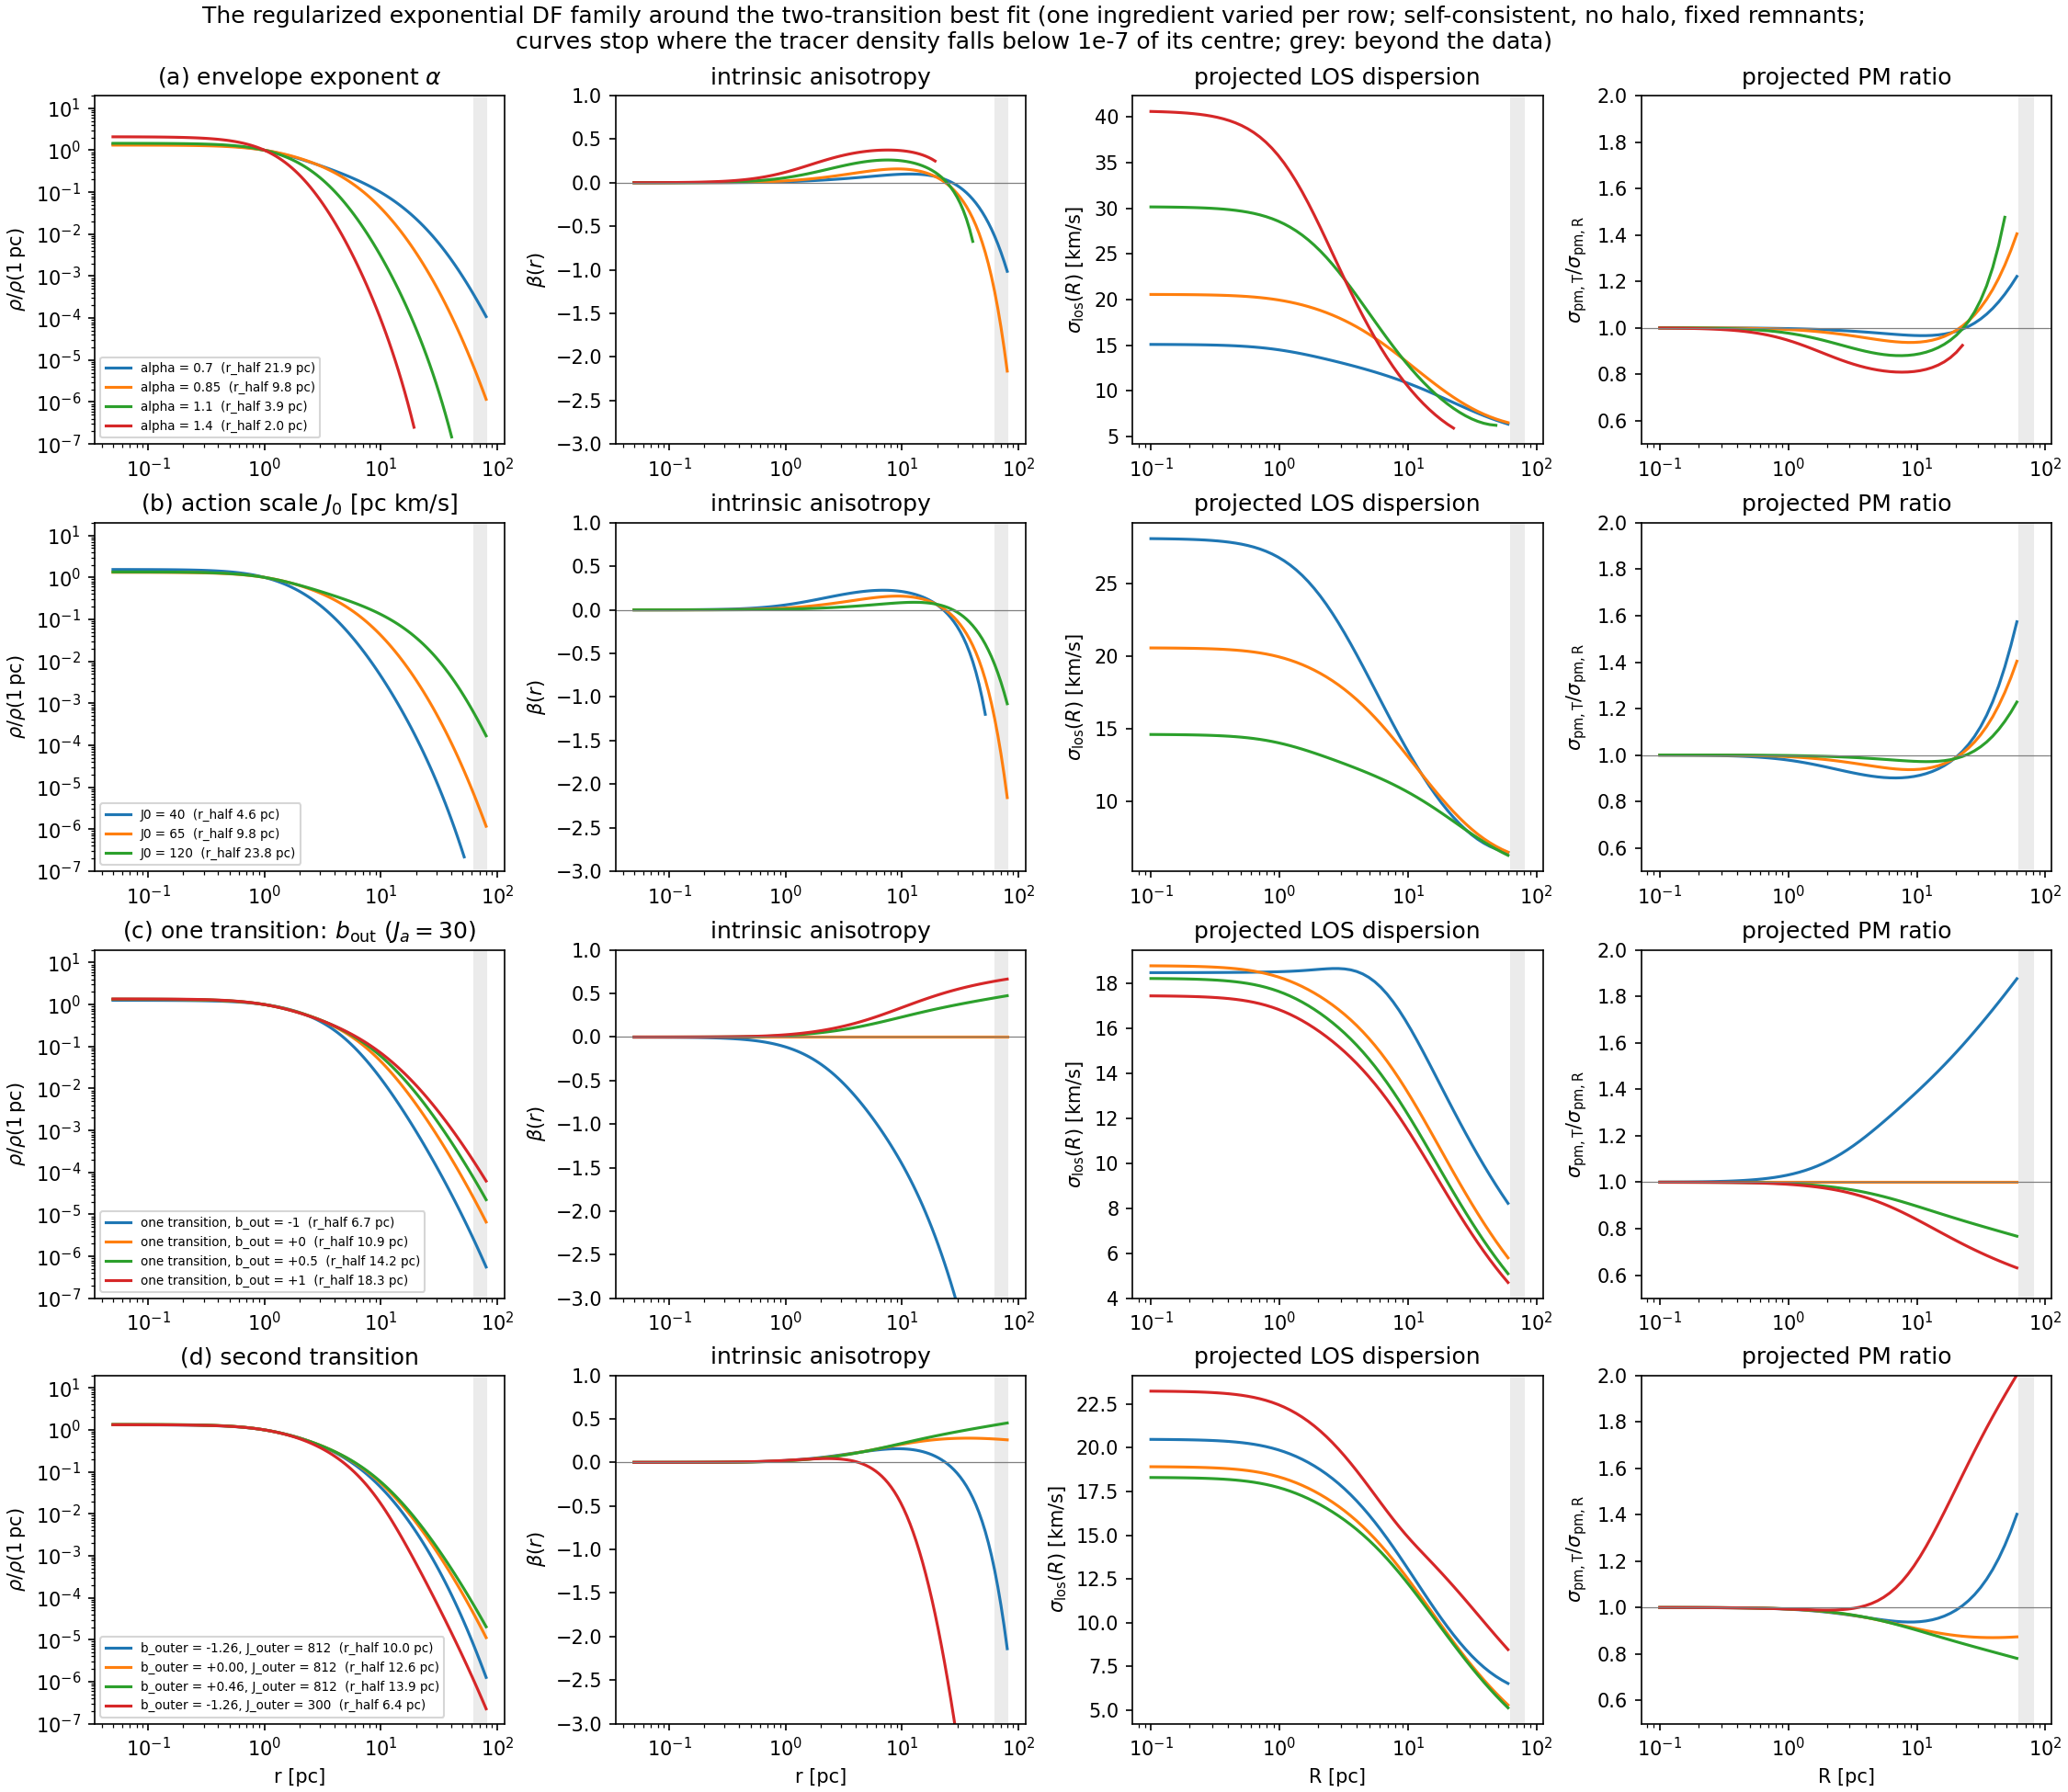
\includegraphics[width=\linewidth]{df_family_gallery_20260923.png}
\caption{The regularized exponential DF family around the two-transition best
fit. Rows vary (a) $\alpha$, (b) $J_0$, (c) a single anisotropy transition
with amplitude $b_{\rm out}$ at $J_a=30\Jact$, and (d) the second transition
($b_{\rm outer}$, $J_{\rm outer}$). All other parameters stay at the best-fit
values. Columns: intrinsic density normalized at 1\pc (legend: half-mass
radius); intrinsic $\beta(r)$; projected $\sigma_{\rm los}(R)$; projected
$\sigma_{{\rm pm},T}/\sigma_{{\rm pm},R}$. Every model is a self-consistent
equilibrium in the fitted remnant potential (no halo, no point mass). Curves
stop where the tracer density falls below $10^{-7}$ of its central value.
Grey marks radii beyond the data. These are illustrations, not fits (script
\texttt{bin/plot\_df\_family\_gallery.py}).}
\label{fig:family}
\end{figure}
\FloatBarrier

\subsection{Dark components}

Dark mass enters as prescribed spherical densities in the same potential:
\begin{itemize}
\item \textbf{Remnants}: a Plummer sphere with mass $M_\remn$ and scale $a_\remn$.
\item \textbf{Halo} (free-halo branch only): a cored profile ($\gamma=0$)
  normalized at 20\pc,
  $\rho_\dm(r)=\rho_{20}\,h(r/r_s)T(r/r_t)/[h(20\pc/r_s)T(20\pc/r_t)]$,
  with $h(x)=(1+x)^{-3}$ and $T(y)=e^{-y^2}$. The scale $r_s$ is free and the
  taper $r_t=1000\pc$ is fixed. The no-halo branch sets $\rho_{20}=0$.
\item \textbf{No central point mass} (Section~\ref{sec:bh}).
\end{itemize}

\subsection{Equilibrium, projection and numerics}

For every trial, the stellar DF is rebuilt and iterated with Poisson's
equation, with the dark densities held fixed, until the stellar density
closes \citep[AGAMA:][]{2019MNRAS.482.1525V}. Projected surface density and
LOS/PM second moments follow from the intrinsic moments, averaged over each
bin's selection nodes. The fitting resolution uses 128 potential nodes, 32
velocity nodes, 240 moment nodes, 128 projection nodes and 192 action-contour
nodes. The equilibrium iteration tolerance is $5\times10^{-5}$
(Section~\ref{sec:numerics}). Every selected solution is validated at doubled
resolution.

\section{Fitting method and validation}
\label{sec:method}

\subsection{Optimizer}

Fits use bounded trust-region least squares (SciPy \texttt{least\_squares},
TRF) on the residual vector of eq.~\eqref{eq:chi2} plus photometry. All
coordinates are scaled to $[0,1]$; mass and action scales are logarithmic.
Jacobians are forward differences with step 0.002, each probe seeded with the
base point's converged stellar potential. The 9--11 probes of a Jacobian run
in parallel worker processes. A fit stops when the objective improves by less
than 0.01 over two accepted steps (well below a meaningful
$\Delta\chi^2\sim1$), when SciPy's own tests are met, or at 600 equilibrium
evaluations. Stops that follow closely after rejected equilibria are recorded
as unconverged. Several starting points are used for each model: two
hand-picked and, for the wide-bound and two-transition runs, four
Latin-hypercube starts (seed 20260923) in the central 60\% of each range.

The second transition is parametrized by $\Delta=\ln(J_{\rm outer}/J_a)\in[\ln2,\ln100]$,
applied after all other coordinates, so $J_{\rm outer}>J_a$ holds for every
trial. The search bounds are listed in Table~\ref{tab:bounds}. They are
optimizer limits, not priors.

\begin{table}[htbp]
\centering\small
\caption{Search bounds. The ``default'' bounds were used in the first batch
only.}
\label{tab:bounds}
\begin{tabular}{lll}
\toprule
Coordinate & Bounds & Notes\\
\midrule
$M_\star$ & $10^6$--$6\times10^6\,\Msun$ (log) & \\
$J_0$ & 30--800\Jact\ (log) & default 100--800\\
$\alpha$ & 0.6--3 & \\
$b_{\rm out}$ & $-2$ to $+2$ & $\pm1$ in one-transition runs\\
$J_a$ & 5--500\Jact\ (log) & default 50--3000; 5--3000 in wide one-transition runs\\
$b_{\rm outer}$ & $-4$ to $+2$ & two-transition only\\
$\ln(J_{\rm outer}/J_a)$ & $\ln2$--$\ln100$ & two-transition only\\
$M_\remn$, $a_\remn$ & $10^2$--$10^6\,\Msun$, 0.3--20\pc\ (log) & \\
$\rho_{20}$, $r_s$ & 0--10\,$\Msun\pc^{-3}$, 5--500\pc\ (log) & free-halo only; default $r_s\le150$\\
\bottomrule
\end{tabular}
\end{table}

\subsection{Numerical checks}
\label{sec:numerics}

\begin{itemize}
\item \textbf{Evaluation noise.} At a converged model, repeating the
  equilibrium with different seeds shifted residuals by up to 0.0060 errors at
  the original tolerance ($5\times10^{-4}$), and Jacobian columns by 0.1--7\%.
  At $5\times10^{-5}$ these fall to 0.00059 errors and 0.01--0.65\%, at 23\%
  higher cost per evaluation. The tighter tolerance is used throughout.
\item \textbf{Parallel Jacobians} reproduce serial ones: all probe objectives
  agree to $2.4\times10^{-9}$ relative. The potential is transferred by file,
  a round trip exact to $3\times10^{-14}$. Probe wall time drops 4.6-fold.
\item \textbf{Validation of each selected fit}: a cold replay, a rebuild at
  doubled resolution, and an independent direct projection over the data
  radii (0.05--68\pc). The thresholds are shifts below 0.1 errors and
  projection agreement within 0.5\%. All solutions reported here pass. The
  largest values are a cold shift of 0.0046, a refinement shift of 0.012
  errors, and a projection difference of 0.11\%.
\end{itemize}

\subsection{Acceptance criteria}

The formal errors are known to be incomplete (Section~\ref{sec:data-issues}),
so structural and statistical success are judged separately.
\begin{itemize}
\item \textbf{Structural pass:} independent starts converge; no coordinate at
  a search bound; no coherent residual pattern; no dataset with $\chi^2/n>3$;
  a physically smooth DF.
\item \textbf{Statistical pass:} $\chikin/N<1.3$, every dataset $\chi^2/n<2$,
  $\chi^2_{\rm phot}/N<2$. This is required only under a justified error
  model; with the published errors it is reported, not required.
\end{itemize}

\section{Results}
\label{sec:results}

\subsection{The one-transition DF fails}
\label{sec:one}

Table~\ref{tab:one} summarizes the one-transition fits. In every branch, all
valid starts converge to the same minimum; five of five do so in each
wide-bound branch. The kinematic fit remains poor. The anisotropy scale $J_a$
sits at its lower bound in every fit, whether that bound is 50 or 5\Jact.
Widening the bounds changes $\chikin$ by only 29 (free halo) and 20 (no
halo). Figure~\ref{fig:one} shows the residual pattern. The tangential PM
dispersion is too high at 3--7\pc (to $-6$ errors) and too low beyond 12\pc
(to $+6$). The LOS dispersion is 3--5 errors too high at 5--8\pc, and the
radial PM 2--5 errors too high beyond 20\pc.

\begin{table}[htbp]
\centering\small
\caption{One-transition fits. The objective is $\chikin+\chi^2_{\rm phot}$
after refinement. Dataset columns give $\chi^2/n$.}
\label{tab:one}
\begin{tabular}{lrrrrrrrrl}
\toprule
Fit & Obj. & $\chikin$ & $\chikin/N$ & HST R & HST T & MUSE & Gaia R & Gaia T & At bound\\
\midrule
Default, free halo & 653.6 & 456.1 & 5.12 & 2.5 & 5.6 & 2.7 & 8.2 & 15.1 & $J_0$, $J_a$, $r_s$\\
Default, no halo & 717.6 & 475.7 & 5.34 & 2.3 & 6.8 & 2.8 & 2.6 & 20.1 & $J_a$\\
Wide, free halo & 623.3 & 427.5 & 4.80 & 2.1 & 4.5 & 2.6 & 10.1 & 13.6 & $J_a$\\
Wide, no halo & 698.1 & 456.1 & 5.12 & 2.1 & 6.2 & 2.7 & 2.6 & 20.2 & $J_a$\\
\bottomrule
\end{tabular}
\end{table}

\begin{figure}[htbp]
\centering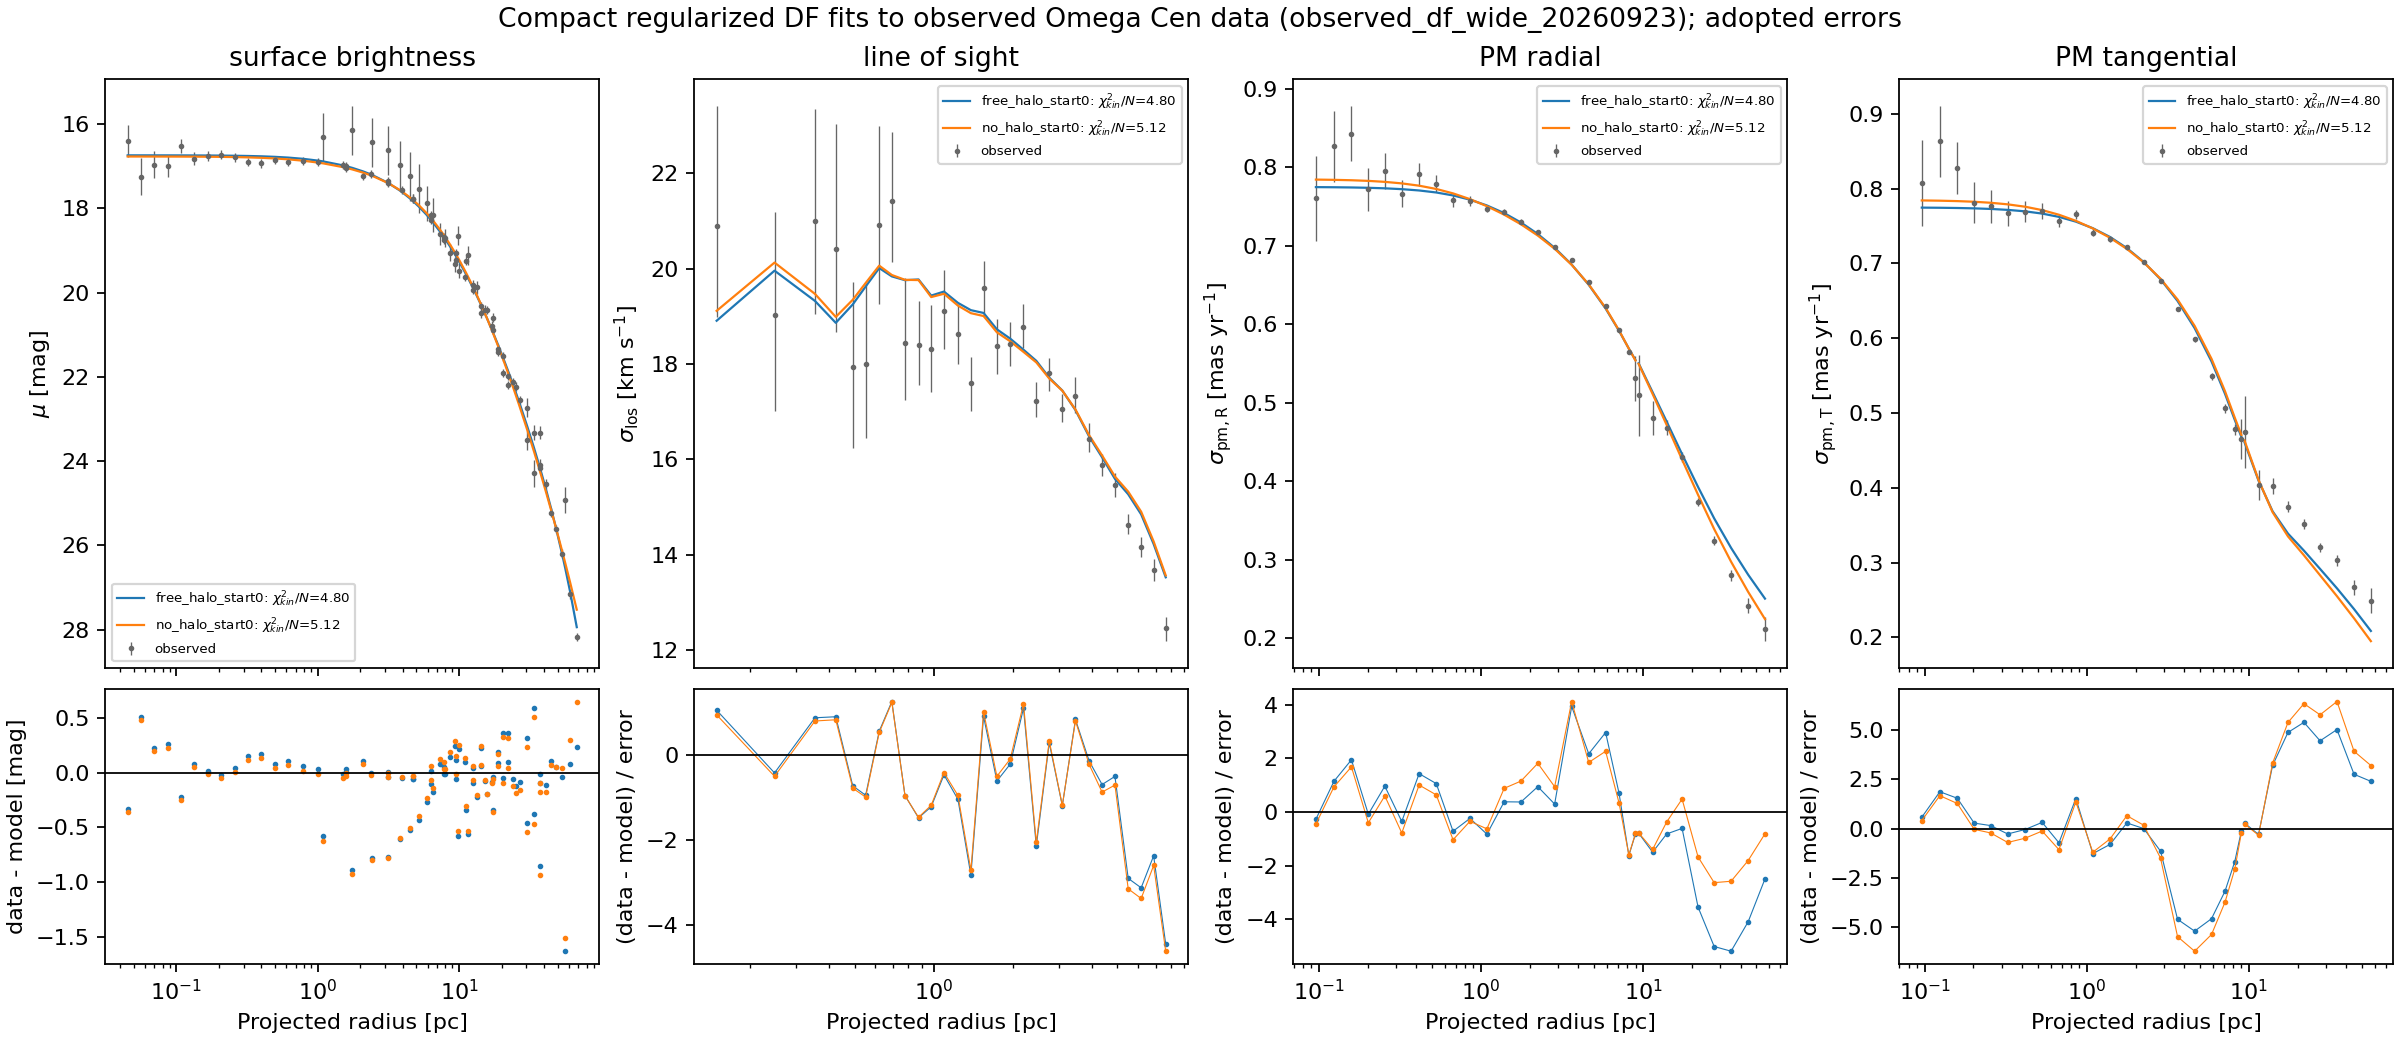
\includegraphics[width=\linewidth]{observed_df_wide_20260923_best_fits.png}
\caption{Best one-transition fits (wide bounds) with and without a halo.
Top: surface brightness, LOS and PM dispersions with published errors.
Bottom: normalized residuals (data$-$model)/error.}
\label{fig:one}
\end{figure}

\subsection{Why it fails: diagnostic fits}
\label{sec:diag}

Diagnostic fits of the same no-halo DF (Table~\ref{tab:diag}) isolate the
cause.

\begin{table}[htbp]
\centering\footnotesize
\caption{Diagnostic fits of the one-transition, no-halo DF. Both starts of
every fit converged to the same solution. The Jeans row is the rung-2
turnover fit (with a point mass, no DM) on the same 89 bins. (b): at a search bound.}
\label{tab:diag}
\begin{tabular}{lrrrrrrrr}
\toprule
Fit & $\chikin/N$ & HST R & HST T & MUSE & Gaia R & Gaia T & $b_{\rm out}$ & $J_a$\\
\midrule
All data & 5.12 & 2.1 & 6.2 & 2.7 & 2.6 & 20.2 & $+0.18$ & 5\,(b)\\
HST+MUSE only (71 bins) & \textbf{1.43} & 1.0 & 1.1 & 2.0 & -- & -- & $+0.39$ & 32\\
Gaia only (18 bins) & \textbf{0.88} & -- & -- & -- & 0.8 & 1.0 & $-1.00$\,(b) & 1665\\
All data, distance free & 4.78 & 1.8 & 6.6 & 1.6 & 2.6 & 19.6 & $+0.18$ & 5\,(b)\\
\emph{Jeans turnover (ref.)} & \emph{2.13} & \emph{2.9} & \emph{1.7} & \emph{1.8} & \emph{1.9} & \emph{2.6} & & \\
\bottomrule
\end{tabular}
\end{table}

\begin{enumerate}
\item \textbf{The DF fits each half of the data.} HST+MUSE and Gaia are each
  fitted well by the same family. Only their combination fails.
\item \textbf{The halves demand opposite anisotropy.} The inner data want
  radial bias switching on at small actions ($b_{\rm out}=+0.39$,
  $J_a=32\Jact$). The outer data want strongly tangential bias
  ($b_{\rm out}=-1$). One transition cannot supply both.
\item \textbf{Distance is not the cause.} Freeing $D$ gives $D=5.30$~kpc and
  lowers $\chikin$ by only 31. Changing $D$ rescales both PM components
  equally and cannot change $\sigma_T/\sigma_R$.
\item \textbf{An independent Jeans fit needs the same shape.} The rung-2 Jeans
  turnover fit prescribes
  $\beta(r)=1-\sigma_t^2/\sigma_r^2$ with two transitions. It finds
  $\beta\simeq+0.15$ near 6\pc, zero near 20\pc, and $-0.6$ to $-0.7$ at
  80\pc. Its central value, $\beta_0=-0.50$, sits at its prior limit
  (Figure~\ref{fig:beta-subsets}).
\end{enumerate}
The tangential turn lies at $\sim20\pc$, inside the Gaia coverage, not at the
HST/Gaia boundary.

\begin{figure}[htbp]
\centering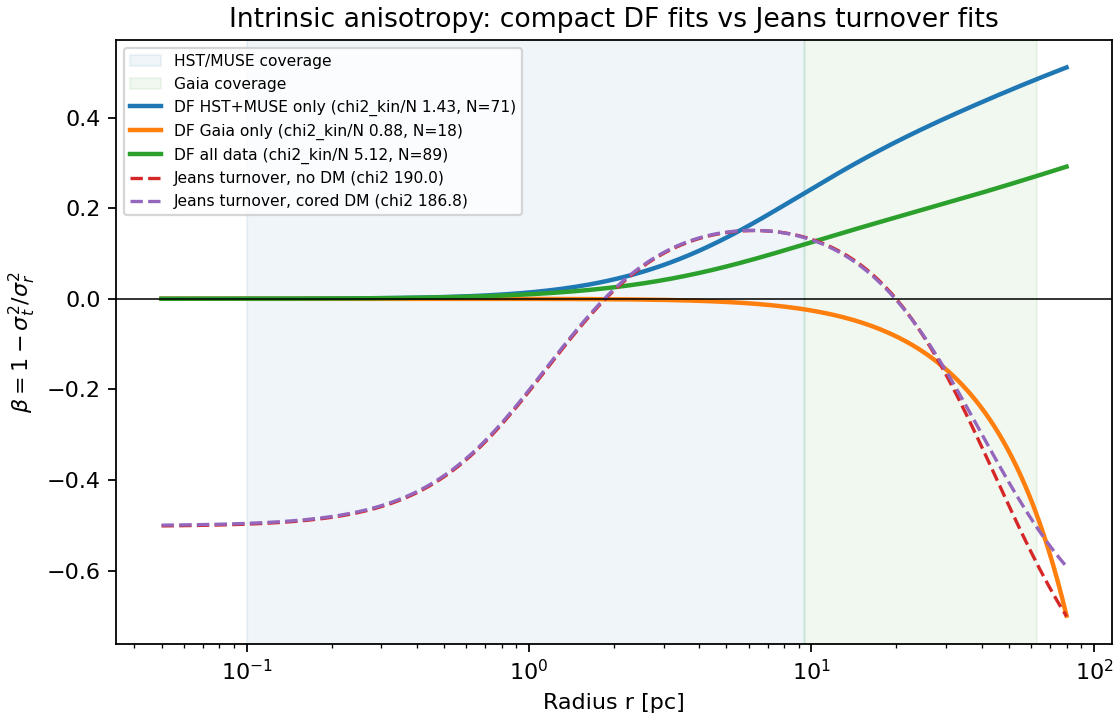
\includegraphics[width=.72\linewidth]{df_subset_beta_20260923.png}
\caption{Intrinsic anisotropy $\beta(r)$ of the one-transition DF fitted to
HST+MUSE only, to Gaia only, and to all data, compared with the rung-2 Jeans
turnover fits. Shading marks the radial coverage of the two surveys.}
\label{fig:beta-subsets}
\end{figure}

\paragraph{Action coverage.} The anisotropy acts on $q=J_r+L$. Sampling
$2\times10^5$ tracers from the best all-data DF shows that the data sample
$q\simeq20$--$730\Jact$ (5--95\%; Figure~\ref{fig:coverage}). The Gaia-only
$J_a=1665$ lies above even the outermost bin's 95th percentile. That fit
therefore used only the low-$q$ tail, $b\simeq b_{\rm out}(q/J_a)^2$, where
only $b_{\rm out}/J_a^2$ is constrained. Neighbouring radial ranges overlap
strongly in $q$, so a transition in $q$ is soft in radius. These results set
the bounds for the second transition (Table~\ref{tab:bounds}).

\begin{figure}[htbp]
\centering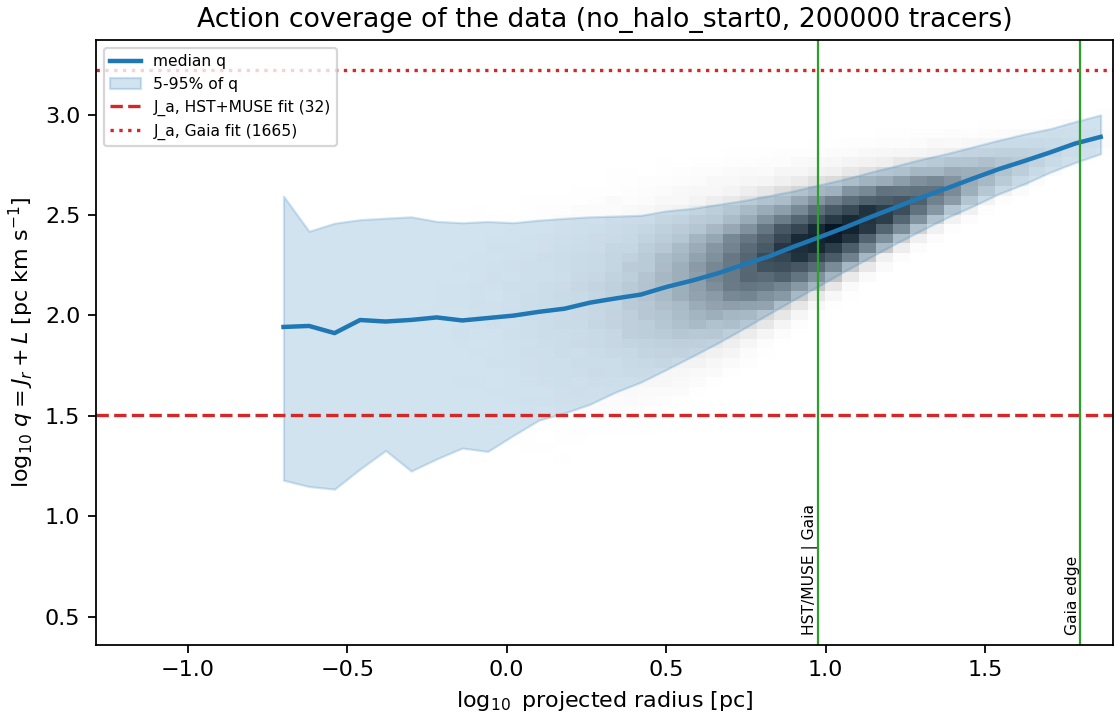
\includegraphics[width=.72\linewidth]{action_coverage_observed_df_wide_20260923.png}
\caption{Distribution of $q=J_r+L$ of DF tracers against projected radius,
with 5--95\% quantiles. Horizontal lines mark the $J_a$ of the HST+MUSE-only
(32) and Gaia-only (1665) fits.}
\label{fig:coverage}
\end{figure}

\subsection{The two-transition DF without a halo}
\label{sec:two}

Six starts were run: the two hand-picked starts combine the two subset
solutions, and four are Latin-hypercube starts. Two Latin starts were
infeasible at their initial point. The four valid starts converged to one
minimum (refined objective 378.3--378.4, $\Delta\chikin\le0.6$), with no
coordinate at a bound and no rejected evaluation. The best-fit parameters are
$M_\star=3.25\times10^6\,\Msun$, $J_0=65\Jact$, $\alpha=0.85$,
$b_{\rm out}=+0.46$, $J_a=27\Jact$, $b_{\rm outer}=-1.26$,
$J_{\rm outer}=812\Jact$, $M_\remn=1.72\times10^5\,\Msun$ and $a_\remn=1.27\pc$.

$\chikin$ falls from 456.1 to \textbf{159.2} ($\chikin/N=1.79$). Gaia
tangential improves from $\chi^2/n=20.2$ to 3.7 (Table~\ref{tab:perf}). The
intrinsic $\beta(r)$ follows the Jeans turnover to $\sim30\pc$
(Figure~\ref{fig:beta-two}): $\beta=0.02$, 0.14, 0.16, 0.06 and $-0.13$ at
1, 6, 10, 20 and 30\pc. Beyond $\sim40\pc$ it falls faster, reaching
$-1.27$ at 63\pc. That region is driven by the $b_{\rm outer}$ asymptote,
which acts only beyond the sampled $q$, so it is an extrapolation. The bias
$b(q)$ peaks at $+0.41$ at $q=103\Jact$, where the HST/MUSE tracers lie
($q$ 5/50/95\% $=56/170/379$). It crosses zero at $q=488$, inside the Gaia
tracers ($183/347/650$; Figure~\ref{fig:structure}). The DF is smooth and
monotonic in the $(J_r,L)$ plane, with no ridge at either transition. The
remnant component returns to the inner-data values: the $6.6\times10^5\,\Msun$
remnant of the Gaia-only fit was compensating for the missing tangential
outskirts.

\begin{figure}[htbp]
\centering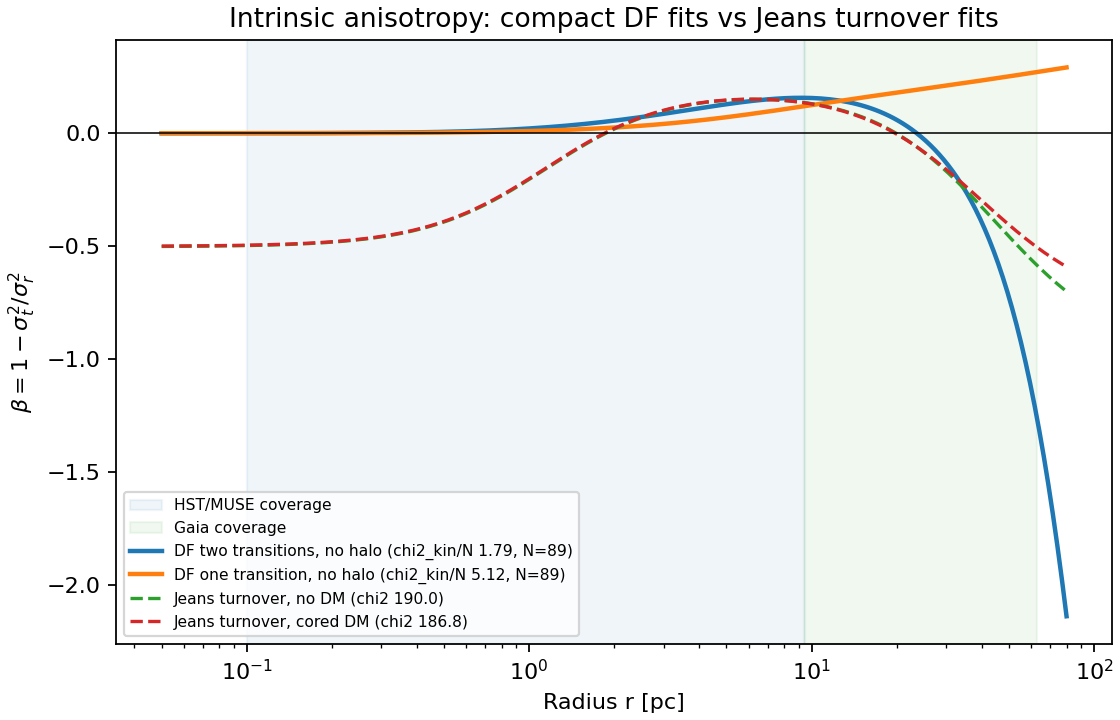
\includegraphics[width=.72\linewidth]{dftwo_beta_20260923.png}
\caption{Intrinsic anisotropy of the two-transition fit (no halo) against the
one-transition fit and the Jeans turnover fits.}
\label{fig:beta-two}
\end{figure}

\begin{figure}[htbp]
\centering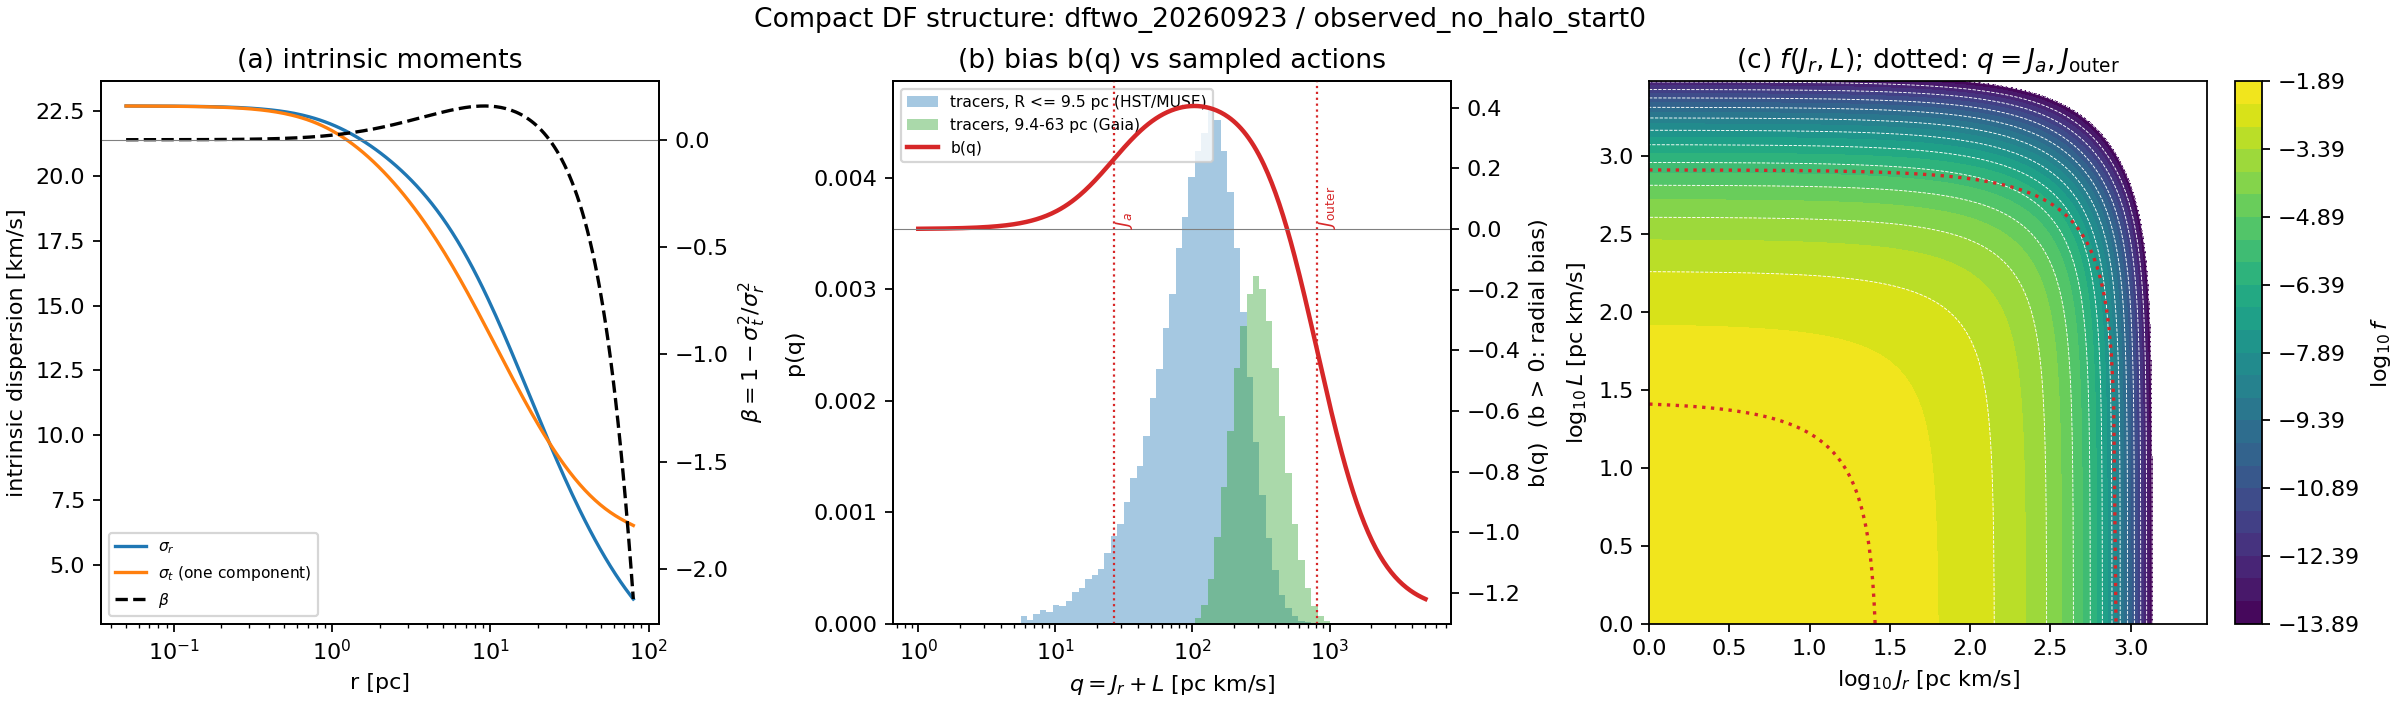
\includegraphics[width=\linewidth]{df_structure_dftwo_20260923_observed_no_halo_start0.png}
\caption{Structure of the two-transition fit (no halo). (a) Intrinsic
$\sigma_r$, one-component $\sigma_t$ and $\beta(r)$. (b) The bias $b(q)$ over
the $q$ distributions of tracers in the HST/MUSE and Gaia projected ranges.
(c) $\log_{10}f$ in the $(J_r,L)$ plane ($J_z=0$); dotted lines mark
$q=J_a$ and $q=J_{\rm outer}$.}
\label{fig:structure}
\end{figure}

\subsection{Adding a free cored halo}
\label{sec:halo}

With a free halo, three of six starts were infeasible at their initial
point: two numerically (an action-normalization error of $5.1\times10^{-5}$
above the $2\times10^{-5}$ tolerance, and a density-closure failure) and one
physically (the streaming term exceeded the DF second moment). The three
valid starts converged to one minimum. The refined objective is 346.9, against
378.3 without a halo, and $\chikin=143.3$. The fitted parameters are
$\rho_{20}=0.92\,\Msun\pc^{-3}$, $M_\star=3.21\times10^6\,\Msun$,
$b_{\rm out}=1.76$, $J_a=101\Jact$, $b_{\rm outer}=-0.25$ and
$J_{\rm outer}=203\Jact$. However:
\begin{itemize}
\item \textbf{Two coordinates are at bounds}: $r_s=500\pc$ (upper), making
  the halo effectively uniform inside the data, and
  $J_{\rm outer}/J_a=2$ (lower), pushing the two transitions together.
\item \textbf{The anisotropy rearranges}: $b_{\rm out}$ changes from $0.46$
  to $1.76$ and $b_{\rm outer}$ from $-1.26$ to $-0.25$.
\item \textbf{The halo acts only in the outskirts}: it is under 1\% of the
  enclosed mass at 20\pc, 8\% at 42\pc and 32\% at 80\pc. It trades misfit
  between the Gaia components: tangential improves from 3.7 to 2.3 while
  radial worsens from 0.9 to 2.0.
\end{itemize}
This is the classic mass--anisotropy trade. The objective gain (31, with
$\Delta\chikin=16$ for two extra coordinates) cannot be read as a DM
preference (Section~\ref{sec:dm}).

\subsection{Performance of the best-fit models}
\label{sec:performance}

Table~\ref{tab:perf} and Figures~\ref{fig:perf-data}--\ref{fig:perf-diag}
summarize the two best fits. The runs test counts sign changes of the
residuals along radius; $z<-2$ means too few runs, i.e.\ coherent residuals.

\begin{table}[htbp]
\centering\small
\caption{Performance of the two-transition fits with published errors.
$p$ is the $\chi^2$ survival probability for $n$ independent bins (indicative
only). The last column gives the largest absolute normalized residual.}
\label{tab:perf}
\begin{tabular}{lrrrrrr}
\toprule
& \multicolumn{2}{c}{no halo} & \multicolumn{2}{c}{free halo} & runs $z$ & max$|r|$\\
Dataset ($n$) & $\chi^2/n$ & $p$ & $\chi^2/n$ & $p$ & (no halo / halo) & (no halo / halo)\\
\midrule
HST PM R (21) & 1.01 & 0.45 & 1.02 & 0.43 & $-0.9$ / $0.0$ & 2.0 / 2.0\\
HST PM T (21) & 1.81 & 0.013 & 1.39 & 0.11 & $-1.1$ / $-1.1$ & 2.6 / 2.1\\
MUSE LOS (29) & 2.01 & 0.001 & 1.84 & 0.004 & $+0.5$ / $+0.5$ & 3.6 / 3.2\\
Gaia PM R (9) & 0.93 & 0.50 & 2.04 & 0.03 & $-2.3$ / $-1.2$ & 1.9 / 2.2\\
Gaia PM T (9) & 3.70 & $10^{-4}$ & 2.34 & 0.01 & $-0.8$ / $-1.0$ & 3.6 / 2.7\\
Photometry (82) & 2.67 & $2\times10^{-14}$ & 2.48 & $3\times10^{-12}$ & $-1.2$ / $-2.1$ & 5.7 / 5.8\\
\midrule
$\chikin$ (89) & \multicolumn{2}{c}{159.2} & \multicolumn{2}{c}{143.3} & & \\
$\chi^2_{\rm phot}$ (82) & \multicolumn{2}{c}{219.1} & \multicolumn{2}{c}{203.6} & & \\
\bottomrule
\end{tabular}
\end{table}

\begin{figure}[htbp]
\centering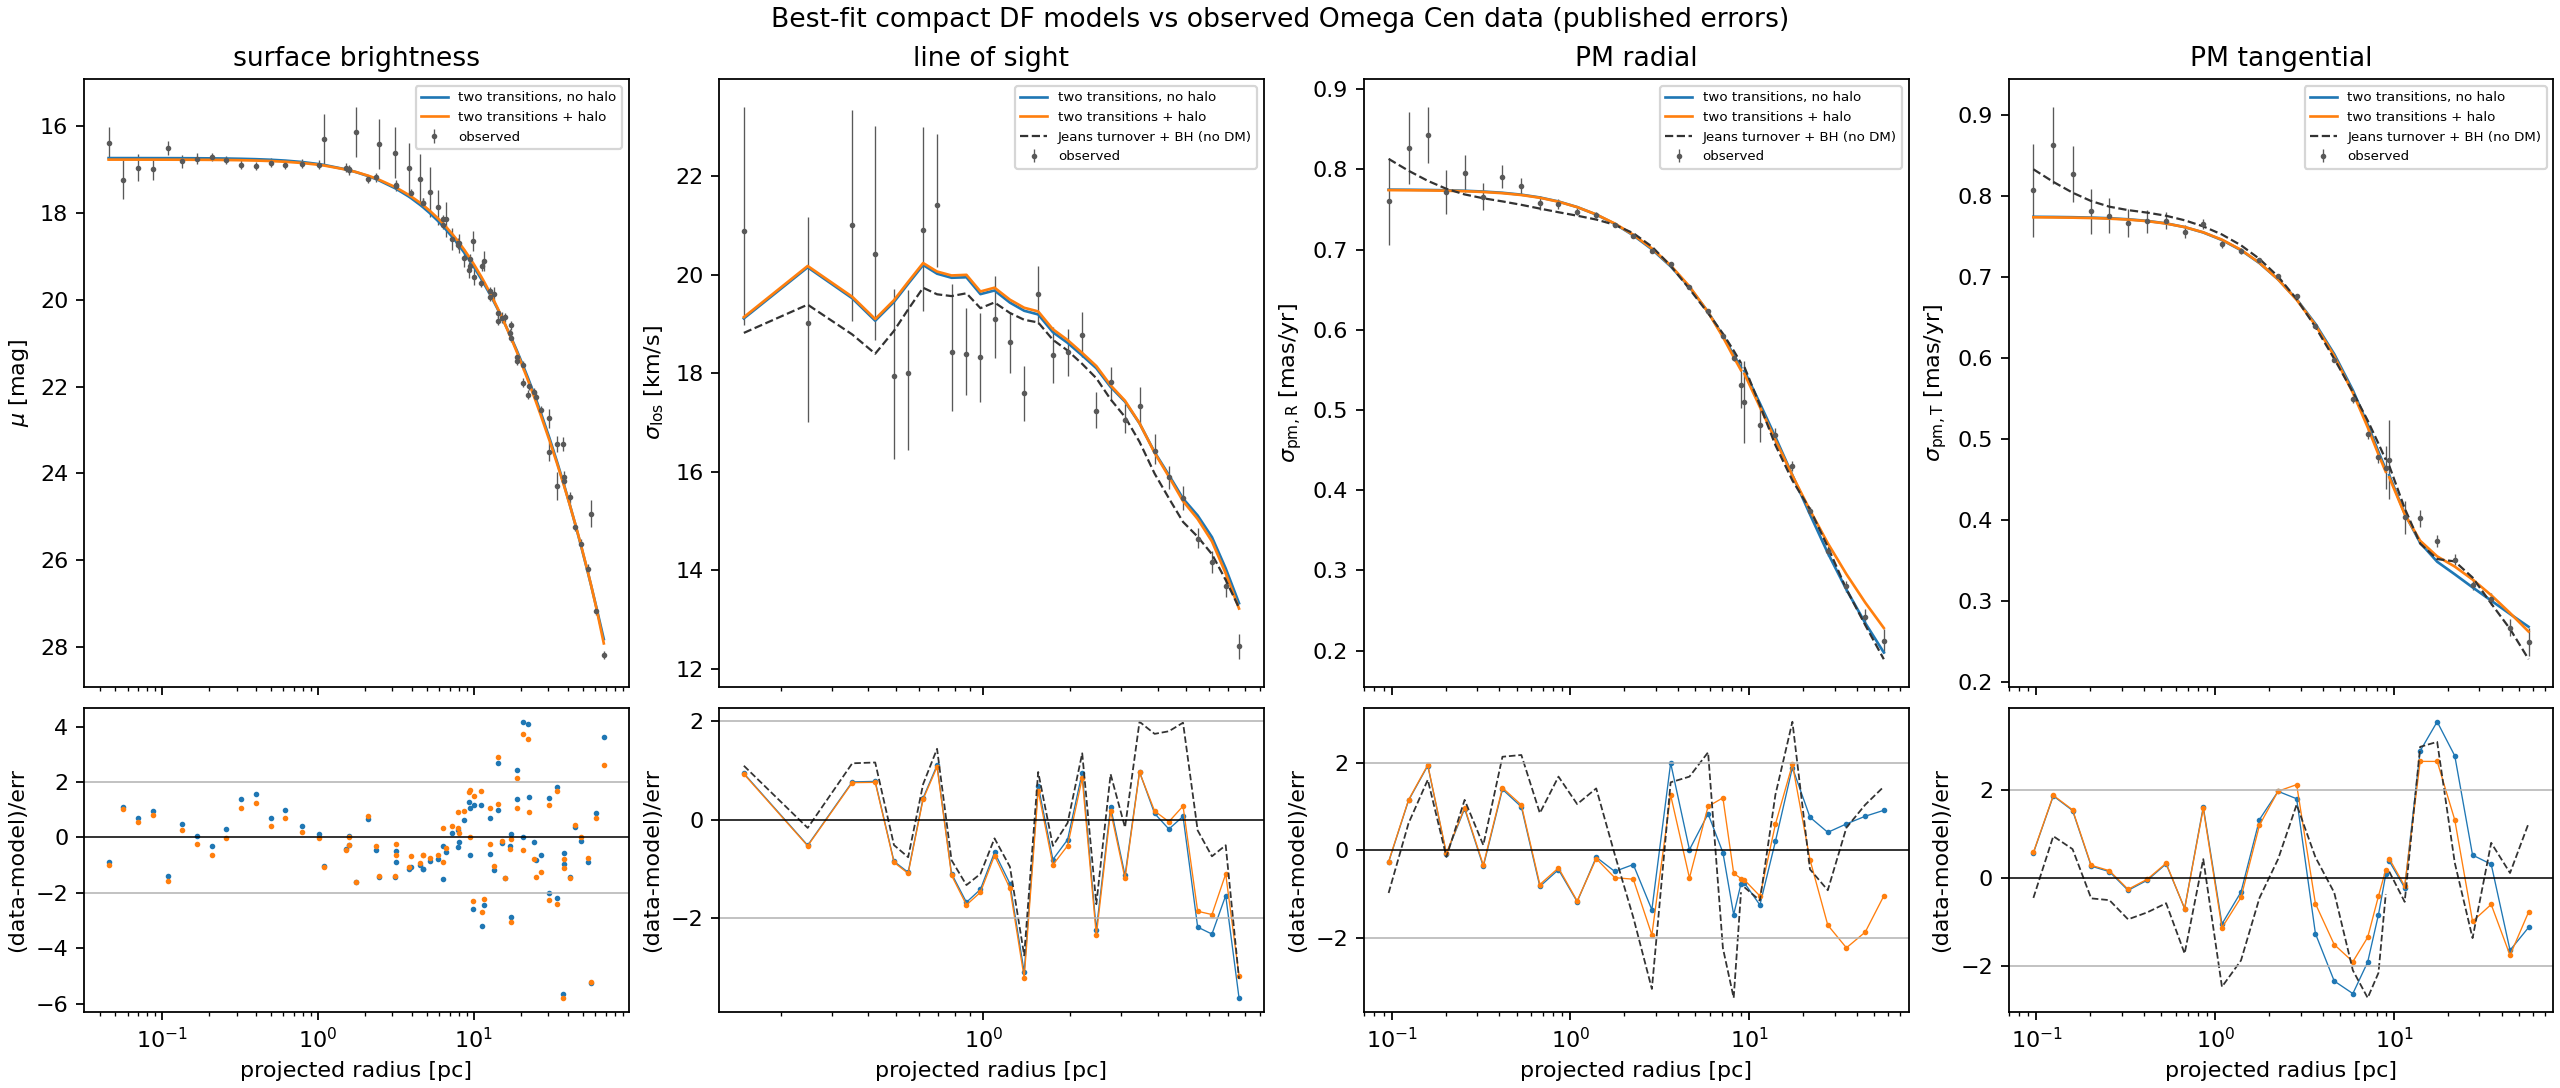
\includegraphics[width=\linewidth]{best_fit_performance_20260923_data.png}
\caption{Best two-transition fits without (blue) and with (orange) a halo,
and the rung-2 Jeans turnover fit (dashed; kinematics only). Bottom:
(data$-$model)/error, with $\pm2$ lines.}
\label{fig:perf-data}
\end{figure}

\begin{figure}[htbp]
\centering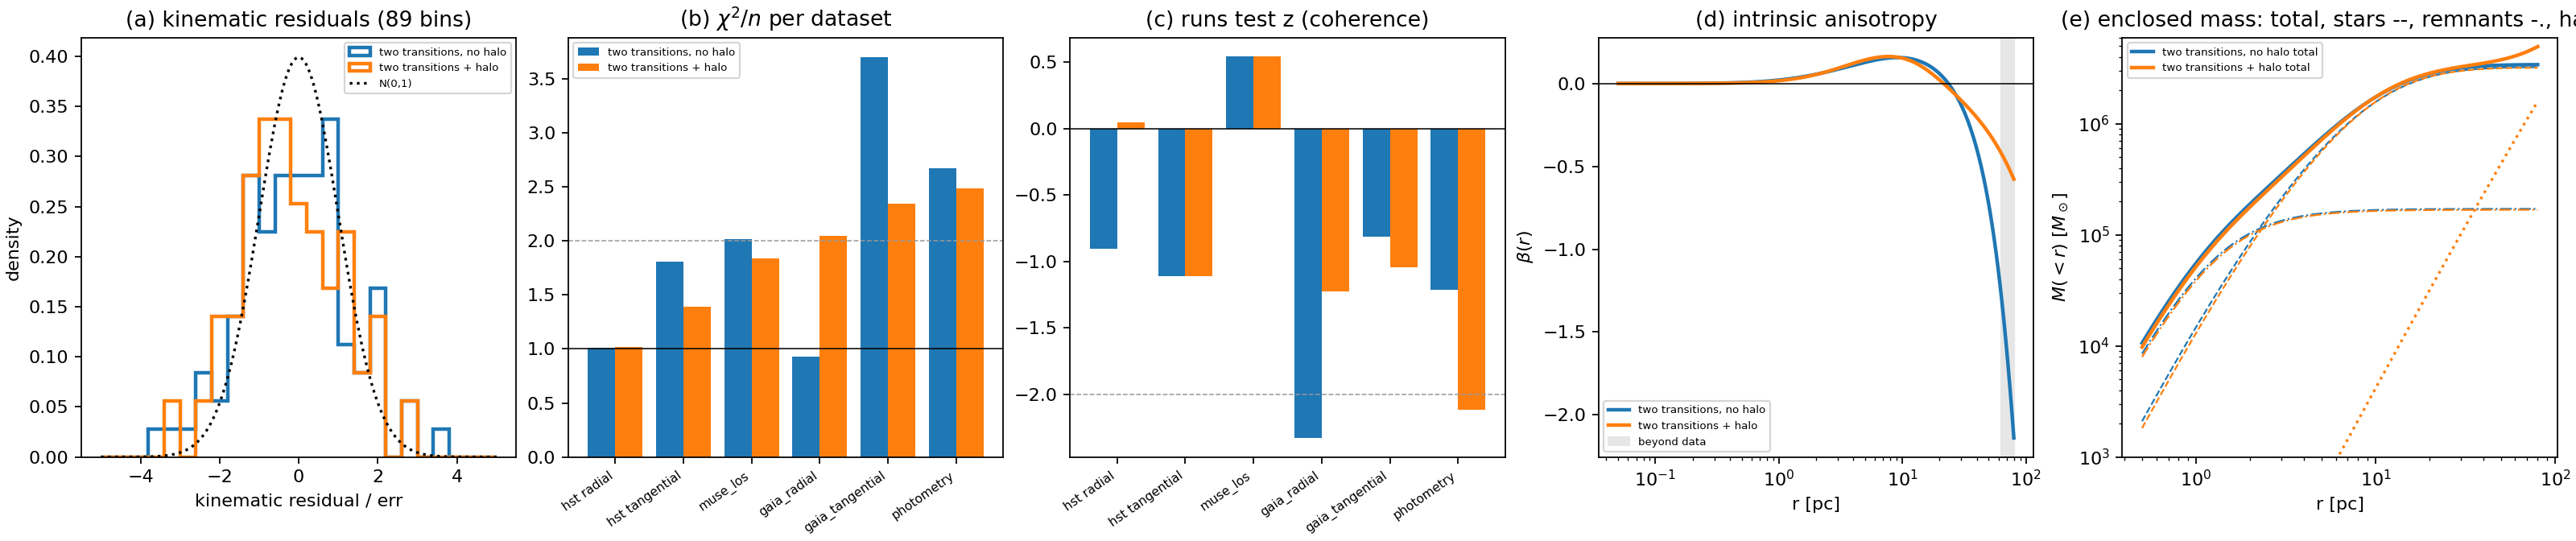
\includegraphics[width=\linewidth]{best_fit_performance_20260923_diagnostics.png}
\caption{Diagnostics of the two best fits: (a) kinematic residuals against
$N(0,1)$; (b) $\chi^2/n$ per dataset; (c) runs-test $z$ per dataset;
(d) intrinsic $\beta(r)$; (e) enclosed mass by component (total, stars,
remnants, halo).}
\label{fig:perf-diag}
\end{figure}

\begin{itemize}
\item \textbf{The kinematics are now fitted better than by the best Jeans
  model} ($\chikin=159.2$ and 143.3, against 190.0), with a positive,
  self-consistent DF. All profiles are tracked over 0.1--63\pc. The residual
  distribution is somewhat wider than $N(0,1)$, with tails to $\pm3.6$.
\item \textbf{The remaining structured misfits are localized.} The MUSE LOS
  is 2--3.6 errors too high at its outer edge (5--8\pc), where the streaming
  correction is largest. The tangential PMs are 2--2.6 errors too high at
  4--7\pc and up to 3.5 errors too low at 15--20\pc (the first Gaia bins).
  With the halo, the outer Gaia radial PM becomes $\sim2$ errors too high.
\item \textbf{The photometric misfit} is dominated by 10--40\pc points with
  residuals of opposite sign at similar radii ($-3$ to $-6$ and $+2$ to $+4$).
  This is consistent with the internal scatter of the compilation
  (Section~\ref{sec:data-issues}); this interpretation has not been tested.
\item \textbf{The two models are nearly identical inside the data}: $\beta(r)$
  and the total $M(<r)$ coincide to $\sim25\pc$.
\end{itemize}

\textbf{Verdict on objective 1.} The two-transition DF is a structural
near-pass. The only structural criterion it misses is Gaia tangential at
$\chi^2/n=3.7$ (without a halo), against a limit of 3. It is not a
statistical pass under the published errors: $\chikin/N=1.79$ and 1.61.

\subsection{The two-transition DF with Poisson counts and the distance prior}
\label{sec:counts-fit}

The same two-transition DF was refitted with the count likelihood of
Section~\ref{sec:counts} and the distance as a coordinate with a Gaussian
prior $5.43\pm0.05$~kpc \citep{2021MNRAS.505.5957B}, entering the objective
as $[(D-5.43)/0.05]^2$. No halo. Four of six starts (two hand-picked, two
Latin) converged to one minimum; two Latin starts were infeasible. The
refined objective is 285.6: $\chikin=158.2$, HST count deviance 98.8 (20
bins), Gaia count deviance 26.3 (12 bins), prior 2.2. No coordinate is at a
bound and the numerical checks pass.

\begin{table}[htbp]
\centering\small
\caption{Counts-based fit (no halo). Kinematic rows: $\chi^2/n$; count rows:
Poisson deviance per bin; $p$ as in Table~\ref{tab:perf}.}
\label{tab:counts-fit}
\begin{tabular}{lrrrr}
\toprule
Dataset ($n$) & value & $p$ & runs $z$ & max$|r|$\\
\midrule
HST PM R (21) & 2.07 & 0.003 & $-1.2$ & 3.3\\
HST PM T (21) & 1.95 & 0.006 & $-2.5$ & 2.8\\
MUSE LOS (29) & 1.31 & 0.12 & $-0.5$ & 2.5\\
Gaia PM R (9) & 1.55 & 0.12 & $-1.2$ & 1.9\\
Gaia PM T (9) & 2.42 & 0.010 & $+0.4$ & 3.0\\
HST counts (20) & 4.94 & $2\times10^{-12}$ & $-1.6$ & 4.8\\
Gaia counts (12) & 2.19 & 0.010 & $-0.6$ & 2.9\\
\midrule
$\chikin$ (89) & 158.2 & & & $\chikin/N=1.78$\\
\bottomrule
\end{tabular}
\end{table}

\begin{figure}[htbp]
\centering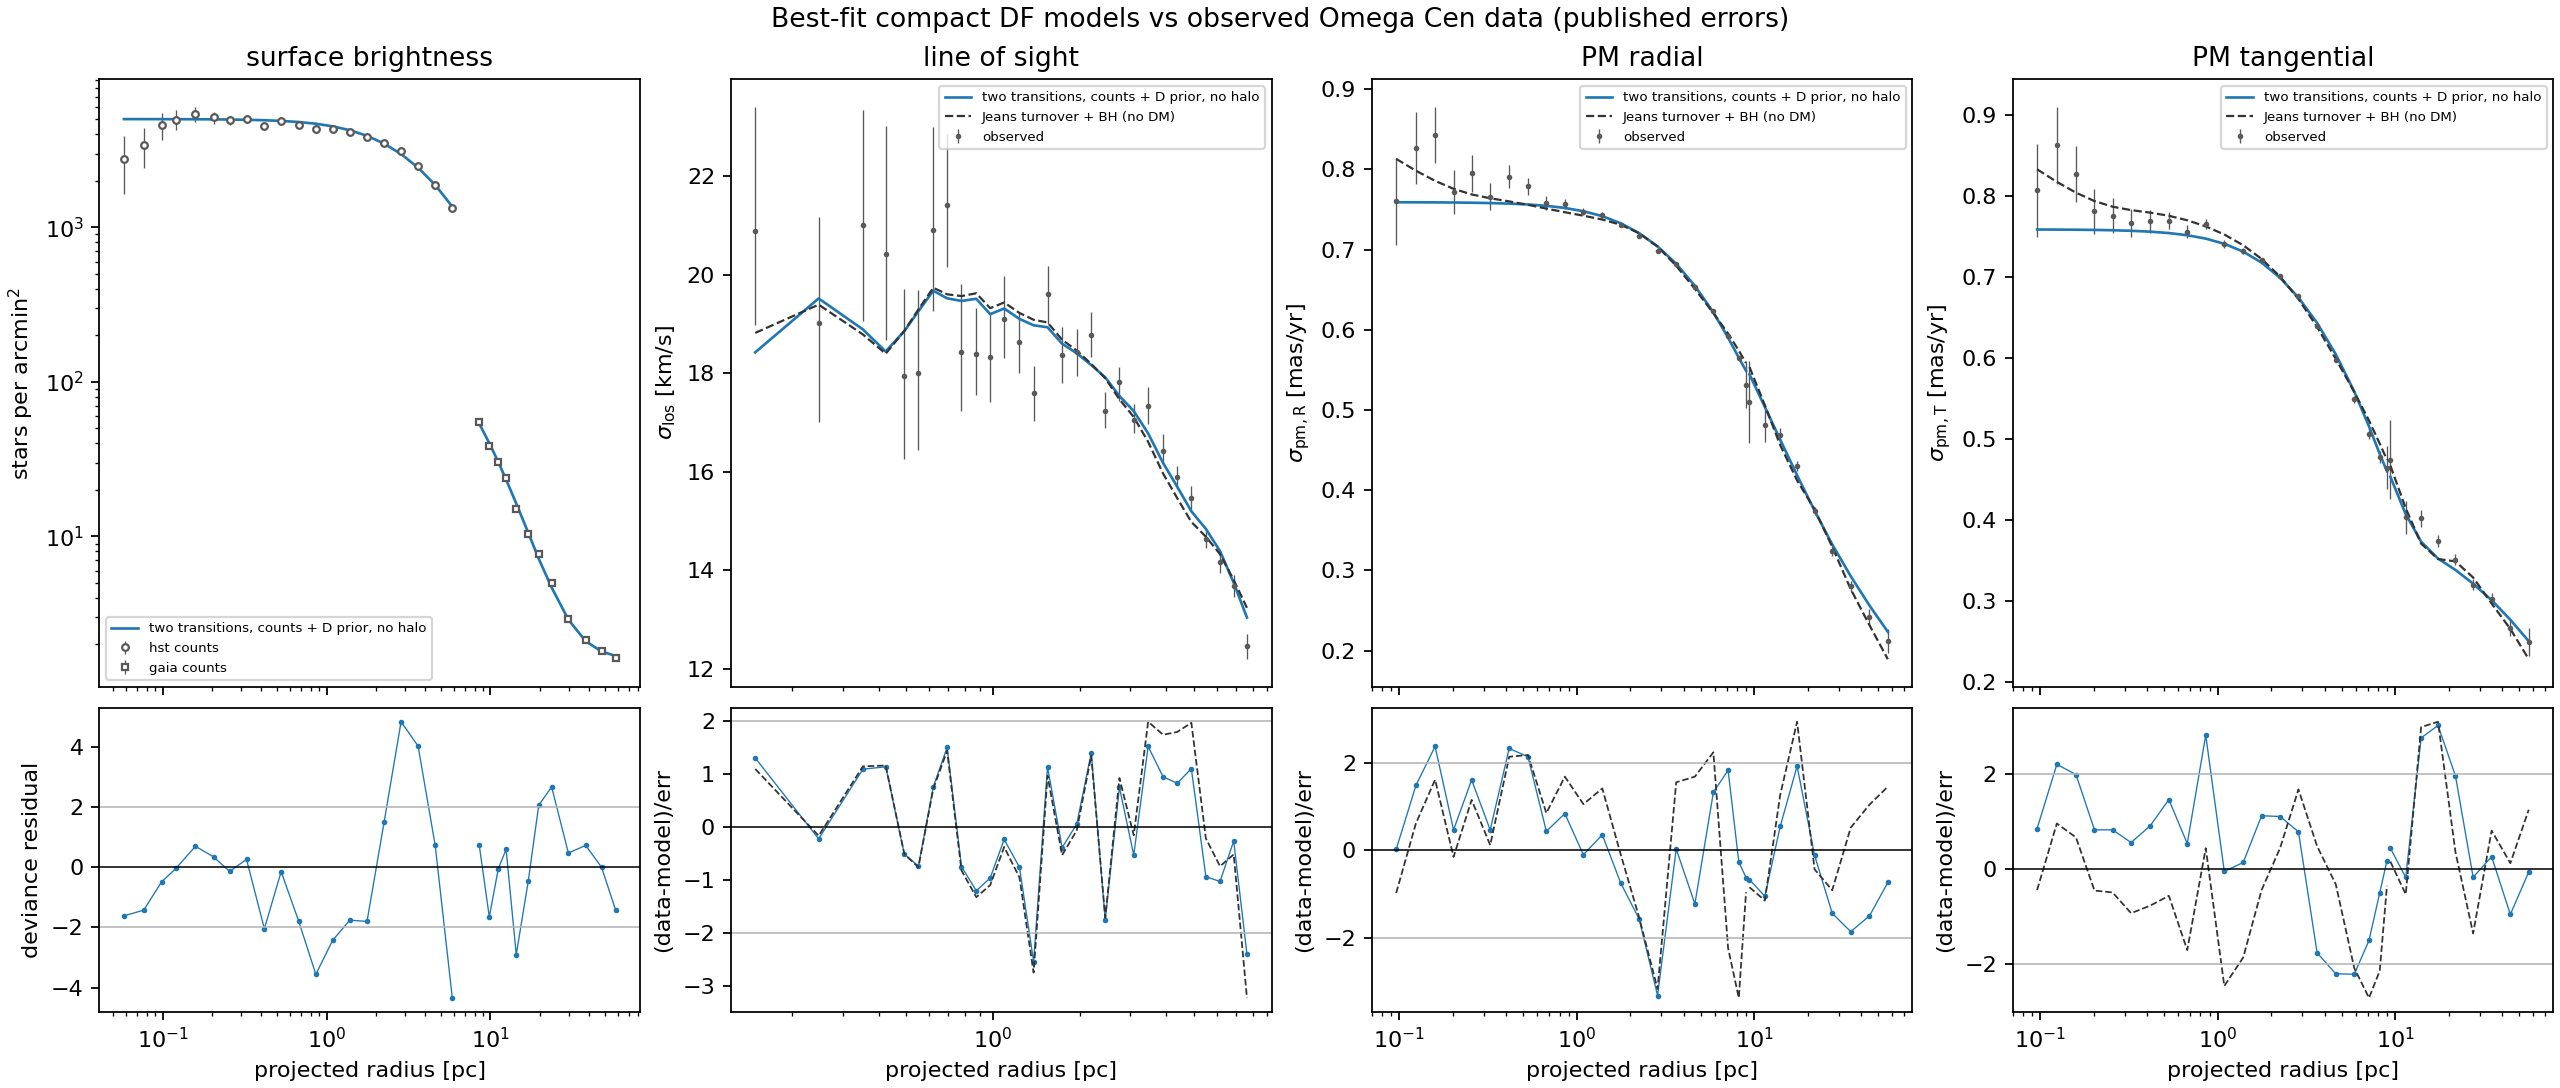
\includegraphics[width=\linewidth]{counts_fit_performance_20260923_data.png}
\caption{The counts-based two-transition fit (no halo). Left: HST and Gaia
surface number densities with Poisson errors and the model $\mu_i/A_i$;
bottom row: deviance residuals for the counts, (data$-$model)/error for the
kinematics. Dashed: the rung-2 Jeans turnover fit (kinematics only).}
\label{fig:counts-fit}
\end{figure}

\begin{itemize}
\item \textbf{Kinematics}: quality unchanged ($\chikin$ 158.2 vs 159.2) but
  more evenly spread: every dataset lies between 1.3 and 2.4 (Gaia
  tangential 2.4, from 3.7). All 89 residuals are within $\pm3.3$ errors.
\item \textbf{Counts}: the Gaia profile is fitted at 2.2 per bin. The HST
  profile, with 118k stars and 0.3--1\% Poisson errors, is the worst-fitted
  term: the model is $\sim4$\% low at 2--4\pc, $\sim4$\% high at 5--6.5\pc,
  and low inside 0.1\pc. This is the one-parameter envelope of
  Section~\ref{sec:family} showing its rigidity at the few-per-cent level.
\item \textbf{Parameters}: $M_\star=3.00\times10^6\,\Msun$, $J_0=54\Jact$,
  $\alpha=0.80$, $b_{\rm out}=+0.74$, $J_a=64\Jact$, $b_{\rm outer}=-0.33$,
  $J_{\rm outer}=319\Jact$, $M_\remn=2.62\times10^5\,\Msun$ at 2.15\pc,
  $D=5.356$~kpc (1.5$\sigma$ below the prior).
\item \textbf{The outer anisotropy changes.} Against the Trager-photometry
  fit ($b_{\rm outer}=-1.26$, $J_{\rm outer}=812$), $\beta(r)$ agrees inside
  30\pc but reaches only $-0.45$ at 80\pc instead of $-2.1$. The steep
  tangential outskirts of Section~\ref{sec:two} were an artefact of the
  arbitrary photometric weighting. The parameter count is unchanged.
\end{itemize}

\subsection{Is a central point mass needed?}
\label{sec:bh}

The model has no central black hole. Figure~\ref{fig:bh} compares the 43
kinematic bins inside 2\pc with the no-BH two-transition DF and the rung-2
Jeans fits, which include a free point mass with maximum-likelihood
$M_\bullet=4.4\times10^4\,\Msun$ (16--84\%: 3.9--$4.6\times10^4$).

\begin{table}[htbp]
\centering\small
\caption{$\chi^2$ of the 43 kinematic bins inside 2\pc.}
\label{tab:bh}
\begin{tabular}{lrrrr}
\toprule
Model & total & HST R (13) & HST T (13) & MUSE (17)\\
\midrule
DF, two transitions, no BH, no halo & \textbf{48.8} & 11.7 & 12.5 & 24.6\\
Jeans turnover + BH, no DM & 59.0 & 21.5 & 16.7 & 20.8\\
Jeans turnover + BH, cored DM & 59.3 & 23.7 & 14.1 & 21.4\\
\bottomrule
\end{tabular}
\end{table}

The binned data give no evidence that the DF needs a point mass. Only two HST
bins (0.12--0.16\pc) lie 1--2 errors above the no-BH model, and the innermost
bin (0.10\pc) lies below it. The comparison is not controlled: the Jeans fits
also differ in anisotropy (with $\beta_0=-0.5$ imposed) and in mass model.
The clean test would be the same DF with and without a BH. The binned profiles
also cannot test the published IMBH evidence. That evidence rests on
individual fast-moving stars inside $\sim0.1\pc$, which set a lower limit of
$\sim8200\,\Msun$ \citep{2024Natur.631..285H}, and those stars are not in
these profiles. Adding a BH is therefore deferred.

\begin{figure}[htbp]
\centering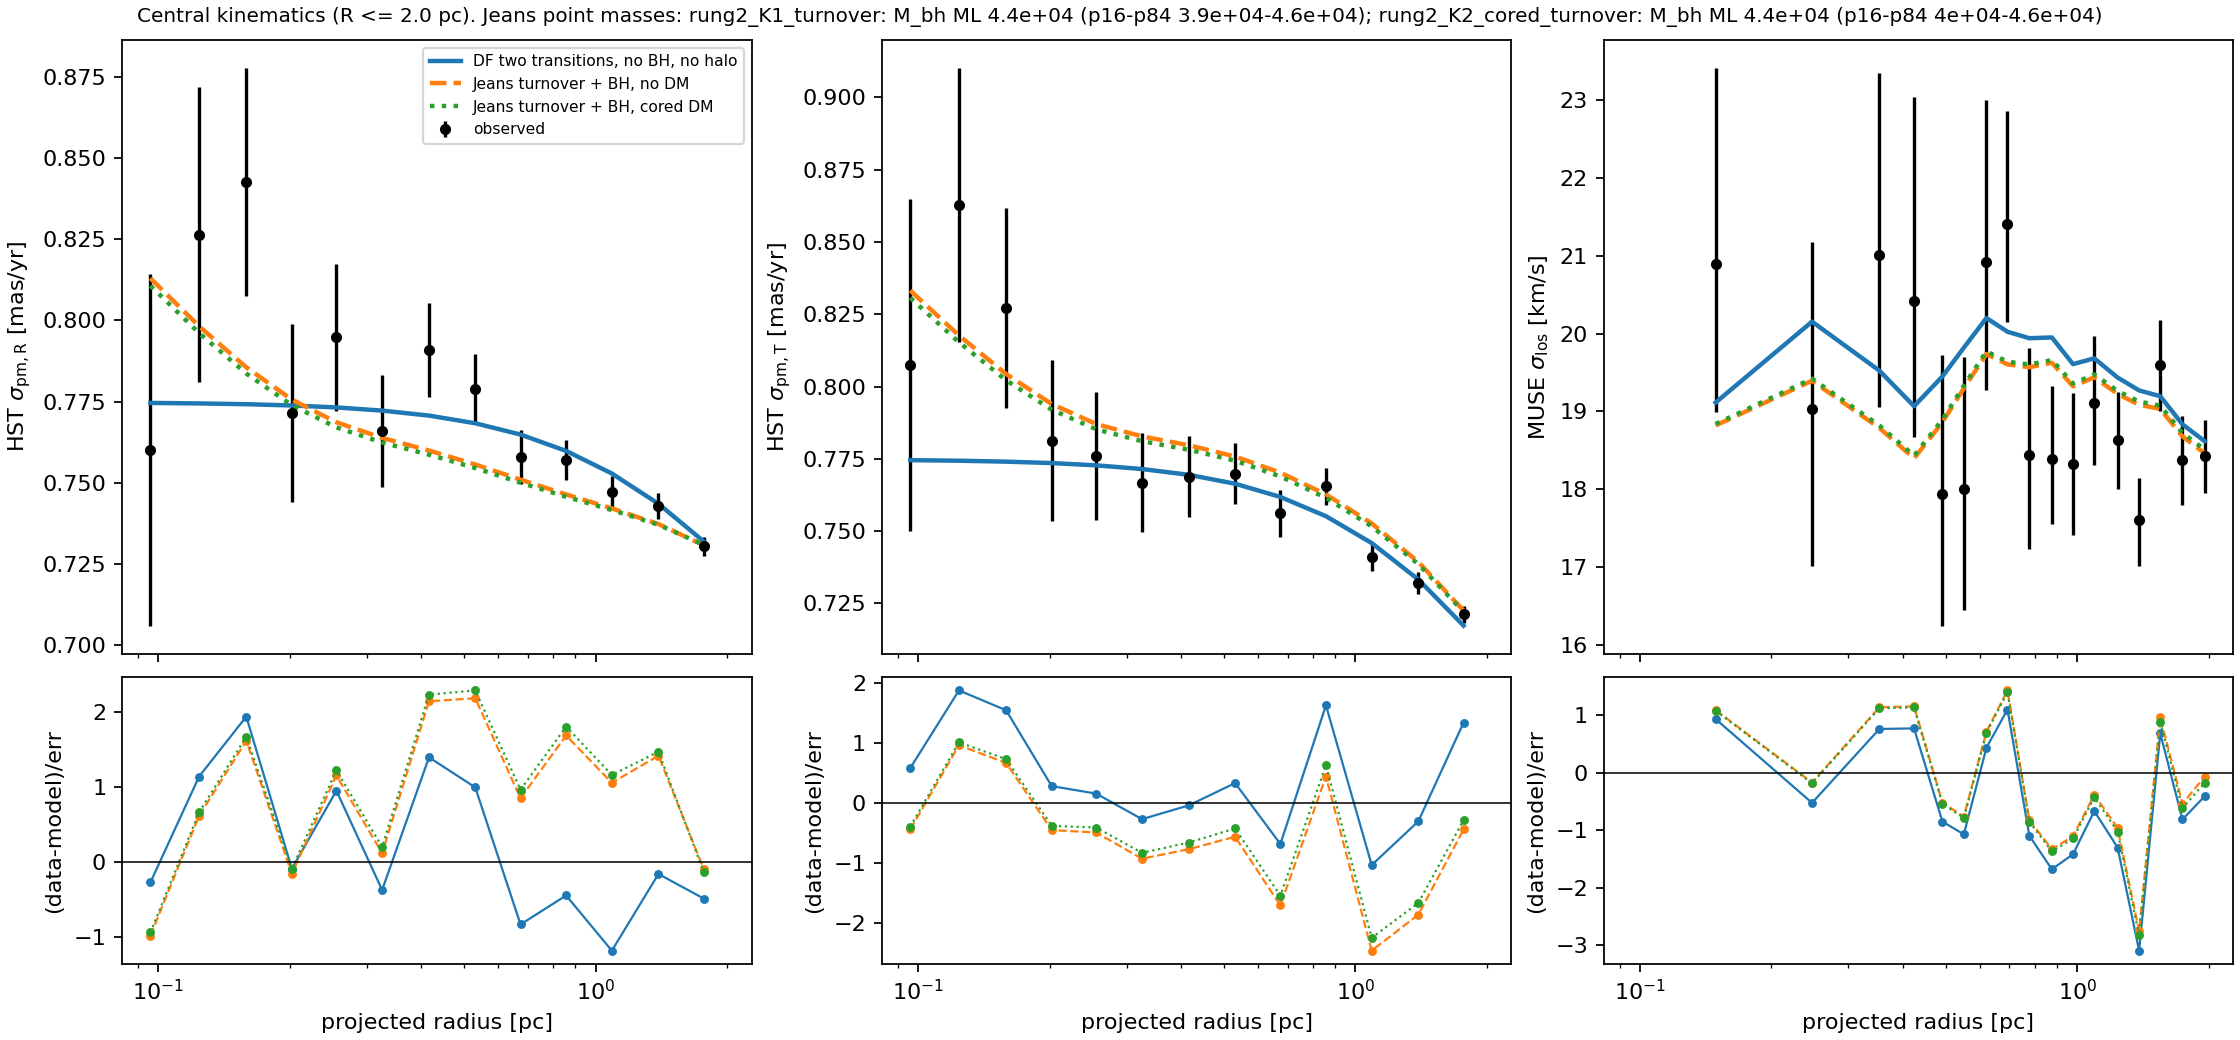
\includegraphics[width=\linewidth]{central_bh_evidence_20260923.png}
\caption{Central kinematics ($R\le2\pc$) with the no-BH two-transition DF and
the Jeans turnover fits with a point mass. Bottom: (data$-$model)/error.}
\label{fig:bh}
\end{figure}

\section{The dark-matter question: what can and cannot be said}
\label{sec:dm}

All statements here use the counts-based likelihood of
Section~\ref{sec:counts-fit}. Earlier halo fits (Section~\ref{sec:halo}) used
the arbitrary photometric weighting and are superseded.

\subsection{Free halo}
With $\rho_{20}$ and $r_s$ free, seeded from the no-halo best fit, the
optimizer converges in 29 evaluations to $\rho_{20}=0$ (at the bound), the
no-halo solution, objective 285.6. The one Latin start was infeasible.

\subsection{Profile likelihood in $\rho_{20}$}
\label{sec:profile}

$\rho_{20}$ was fixed at 0.25, 0.5, 1, 2 and 4\,$\Msun\pc^{-3}$ and every
other coordinate, including $r_s$ (5--500\pc), the anisotropy and the
distance, refitted from the best fit plus one Latin start
(Table~\ref{tab:profile}, Figure~\ref{fig:profile}).

\begin{table}[htbp]
\centering\small
\caption{Profile likelihood in $\rho_{20}$. $\Delta$ is the refined objective
minus its minimum. Halo masses are for the profiled halo. For
$\rho_{20}=0.25$--2 only the seeded start converged (the Latin start was
infeasible); at 4 the Latin start improved the objective from 297.1 to 296.1.}
\label{tab:profile}
\begin{tabular}{rrrrrrrl}
\toprule
$\rho_{20}$ & $\Delta$ & $\chikin$ & counts dev. & $r_s$ [pc] & $M_\dm(<20\pc)$ & $M_\dm(<63\pc)$ & $M_\star$\\
\midrule
0 (free halo) & 0 & 158.2 & 125.2 & -- & 0 & 0 & $3.00\times10^6$\\
0.25 & $+0.51$ & 158.9 & 125.0 & 5 (bound) & $2.4\times10^4$ & $6.2\times10^4$ & $2.96\times10^6$\\
0.5 & $+1.05$ & 159.3 & 125.1 & 5 & $4.8\times10^4$ & $1.2\times10^5$ & $2.92\times10^6$\\
1 & $+2.20$ & 161.1 & 124.4 & 5 & $9.6\times10^4$ & $2.5\times10^5$ & $2.83\times10^6$\\
2 & $+4.78$ & 164.4 & 123.6 & 5 & $1.9\times10^5$ & $4.9\times10^5$ & $2.67\times10^6$\\
4 & $+10.55$ & 171.0 & 122.7 & 5 & $3.8\times10^5$ & $9.8\times10^5$ & $2.35\times10^6$\\
\bottomrule
\end{tabular}
\end{table}

\begin{figure}[htbp]
\centering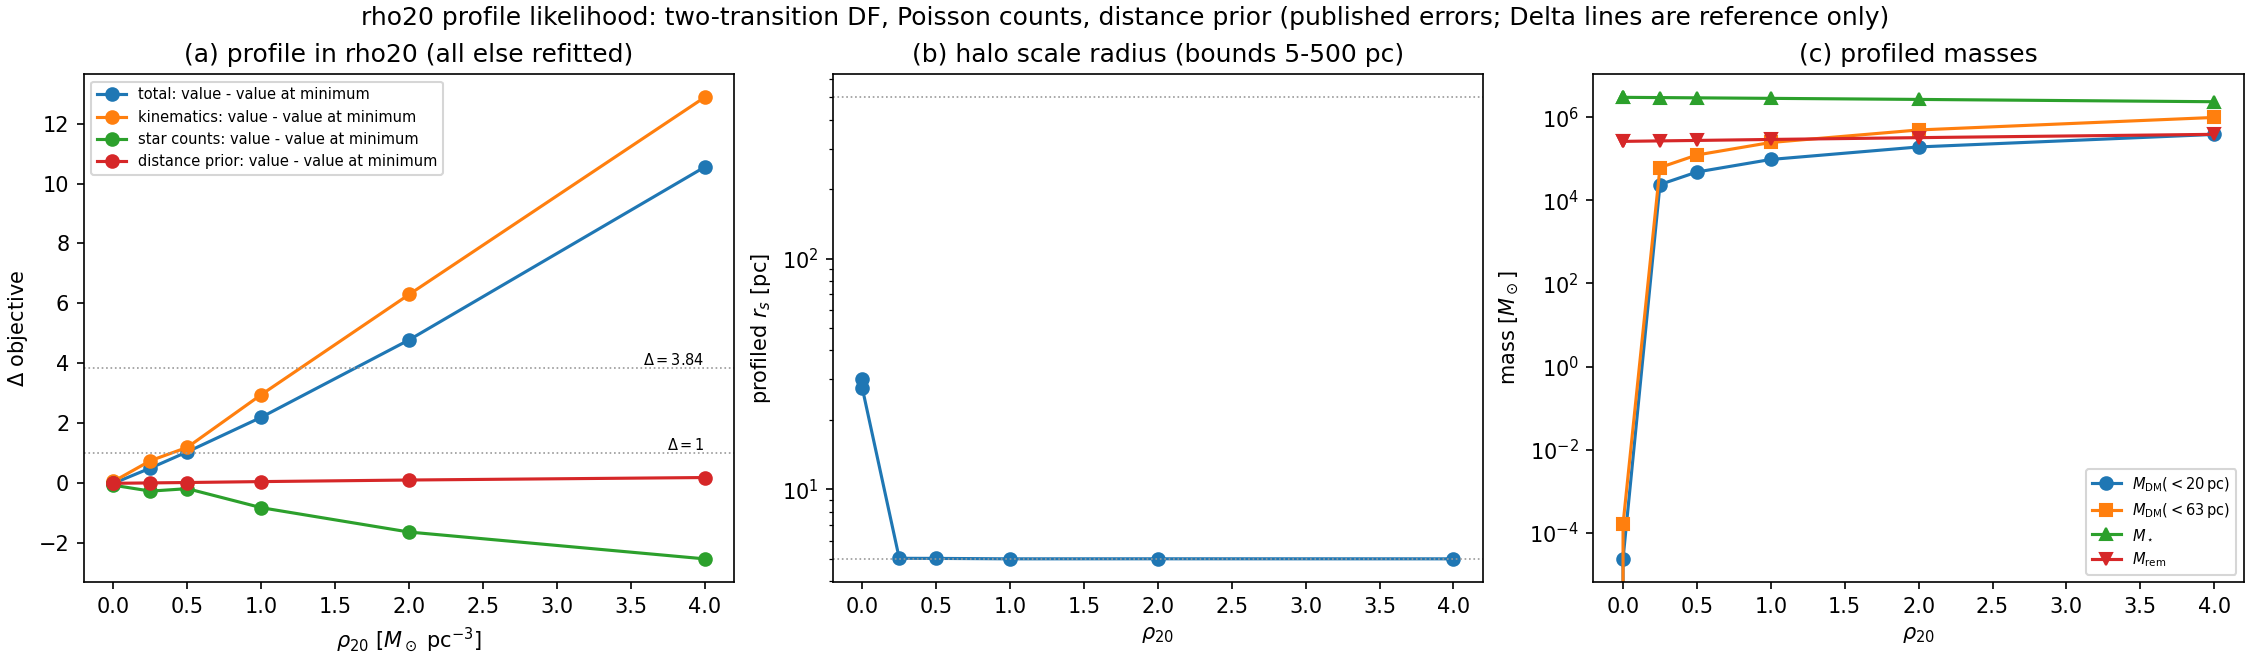
\includegraphics[width=\linewidth]{rho20_profile_20260923.png}
\caption{(a) The objective and its components relative to the minimum
against $\rho_{20}$; the $\Delta=1$ and 3.84 lines are reference values, not
calibrated intervals. (b) The profiled $r_s$. (c) Profiled masses.}
\label{fig:profile}
\end{figure}

\begin{itemize}
\item \textbf{The data prefer no halo, monotonically.} The cost of a forced
  halo comes entirely from the kinematics; the count deviance falls slightly
  and the stellar mass drops from 3.0 to $2.35\times10^6\,\Msun$ across the
  scan: the star/DM trade, now quantified.
\item \textbf{Reference values.} On a $\chi^2$ scale, $\Delta=1$ falls near
  $\rho_{20}\simeq0.5$ and $\Delta=3.84$ near $\rho_{20}\simeq1.7$
  ($M_\dm(<20\pc)\simeq1.6\times10^5\,\Msun$). These would be 68\% and 95\%
  one-parameter limits only under a calibrated likelihood.
  $\chikin/N=1.78$ says the published errors are not, so the real limits are
  looser. No rescaling has been applied.
\item \textbf{The halo is profiled to its least visible shape.} $r_s$ runs to
  the 5\pc bound at every fixed $\rho_{20}$: with the density normalized at
  20\pc, a compact halo has the least mass inside the data. The profile is
  therefore a constraint on the least harmful halo per $\rho_{20}$. A
  physically motivated extended remnant would be constrained more strongly;
  no such prior is imposed, because no clear expectation for $r_s$ exists.
\item \textbf{Comparison.} The earlier Jeans posterior gave a 95\% upper
  limit $\rho_{20}=1.03$ under different assumptions; the two methods agree
  on the order of magnitude.
\end{itemize}

\subsection{Mock validation}
\label{sec:mocks}

Two mocks were built from the counts-based best fit, each with the
published kinematic noise (Gaussian, per bin) and Poisson counts drawn with
the fitted amplitudes: truth A is the fitted model itself ($\rho_{20}=0$);
truth B adds a halo with $\rho_{20}=1$, $r_s=30\pc$. Both were fitted with a
free halo from the generic hand-picked starts, never from the truth.
\begin{itemize}
\item \textbf{A (no halo):} one start recovers $\rho_{20}=0.001$, $M_\star$
  within 0.5\% and the total mass within 1.5\%. The other lands at
  $\rho_{20}=0.12$ with $r_s$ at the 500\pc bound, at the same objective
  within 0.1: a diffuse $\rho_{20}\sim0.1$ halo is indistinguishable from
  none, matching the flat foot of the observed profile.
\item \textbf{B ($\rho_{20}=1$):} both starts give $\rho_{20}=0.79$
  ($-21$\%), $M_\star$ $+3$\%, $M_\remn$ $-20$\%, $r_s$ 260--490\pc
  (unconstrained). The offset lies inside the $\Delta=1$ half-width
  ($\sim0.5$) of the observed profile, so it is consistent with noise on
  one realization.
\end{itemize}
The machinery does not manufacture a halo where there is none and detects
one of $\rho_{20}=1$ when present; it does not recover $r_s$. A coverage test
with five noise seeds per truth is running at the time of writing and will
be added.

\subsection{What can and cannot be said}
\begin{itemize}
\item \textbf{Can:} under this model (spherical, non-rotating, one tracer with
  mass following light, two anisotropy transitions, cored halo with
  $r_s\ge5\pc$) and the published errors, there is no evidence for a DM
  halo, and $\rho_{20}\gtrsim1$--2\,$\Msun\pc^{-3}$ is disfavoured at the
  $\Delta\gtrsim2$--4 level.
\item \textbf{Cannot:} claim an exclusion. The likelihood is not calibrated;
  the recovery test has one realization; rotation is subtracted, not
  modelled; and the tracer/mass assumption is untested. A DM component more
  compact than 5\pc is degenerate with the stellar remnants.
\end{itemize}

\section{Numerical and software issues found and fixed}
\label{sec:fixes}

\begin{itemize}
\item \textbf{Optimizer budget and tolerances.} The first recovery batch
  capped fits at 180 evaluations, about 18 Gauss--Newton steps with nine
  coordinates. Its relative tolerances were tighter than the evaluation
  noise. An absolute stopping rule, a 600-evaluation cap and a tenfold
  tighter equilibrium tolerance fixed both problems.
\item \textbf{Rejected equilibria in Jacobians.} A rejected probe previously
  entered as a $10^6$ residual. That corrupted the Jacobian and collapsed the
  trust region to a spurious ``converged'' stop. Rejected probes are now
  retried in the opposite direction (the column is zeroed if both fail), and
  stops close to rejections are flagged. Infeasible starting points are
  recorded instead of crashing.
\item \textbf{Projection check range.} A 0.8\% fast-vs-direct projection
  difference occurred only at 80\pc, beyond the data (68\pc). Validation now
  covers the data radii.
\item \textbf{Test isolation.} One test module set AGAMA's global units to
  kpc, so later DF tests refused to run (25 failures and errors in the full
  suite). A fixture now restores units; the full suite passes (630 passed,
  5 skipped).
\item \textbf{Remaining numerical limitation.} In strongly DM-dominated
  regions ($M_\star\sim1.4\times10^6\,\Msun$, $\rho_{20}\sim8$) the
  self-consistency iteration can diverge. The normalization tolerance also
  rejected some extreme starts. Neither affects the minima reported here.
\end{itemize}

\subsection*{Withdrawn: Gaia error floors}
\label{sec:floors}
Two diagnostic fits added 0.01 and 0.02\masyr\ in quadrature to the Gaia
errors. They showed that the size of the combined misfit depends strongly on
the Gaia errors ($\chikin/N$ falls from 5.12 to 2.09 with 0.02\masyr),
while the anisotropy conflict persists. Such floors are ad hoc, not a
calibrated error model. They have been withdrawn from all model assessment
and will not be used. The error-model question is left to a separate,
calibrated treatment.

\section{Conclusions and next steps}
\label{sec:conclusions}

\begin{enumerate}
\item The single-transition regularized DF cannot fit the combined $\omega$
  Cen data. The inner and outer data demand radial and tangential anisotropy
  respectively. This is established by converged multi-start fits, subset
  fits and an independent Jeans analysis.
\item The two-transition DF, with no halo and no BH, fits the kinematics
  better than the best existing Jeans model ($\chikin=159.2$ vs 190.0 for
  89 bins). Its anisotropy follows the Jeans turnover inside $\sim30\pc$, and
  its DF is smooth. It is a structural near-pass, not a statistical pass.
\item The remaining misfits are localized at the MUSE outer edge and in the
  4--20\pc tangential PMs, where the rotation correction is largest. The
  photometric misfit appears to be dominated by internal scatter in the
  compilation.
\item Replacing the adopted-error photometry by Poisson star counts leaves
  the kinematic fit unchanged, removes the artificial outer anisotropy, and
  exposes a few-per-cent rigidity of the envelope in the HST counts.
\item With the count likelihood and the distance prior, a free halo goes to
  $\rho_{20}=0$ and the profile likelihood rises monotonically:
  $\Delta=+2.2$ at $\rho_{20}=1$ and $+10.6$ at 4\,$\Msun\pc^{-3}$, for the
  most compact halo allowed. Single-realization mocks recover a no-halo
  truth and detect an injected $\rho_{20}=1$ at 0.79. This is a provisional,
  uncalibrated upper limit of order $\rho_{20}\sim1$--2, not an exclusion.
\end{enumerate}

\paragraph{Objective 1 (fit), proposed.}
(i) Model rotation with an odd-$L_z$ DF component and fit the mean
velocities jointly, instead of subtracting published curves.
(ii) Calibrate the Gaia (and HST) error models from literature systematics
or from the HST/Gaia overlap, as a separate data task whose method needs
approval.
(iii) Examine the photometric compilation for internally inconsistent
sources.
A central BH, separate tracer and mass DFs, and an axisymmetric DF remain
later options, to be introduced only when the data demand them.

\paragraph{Objective 2 (DM), proposed.}
(i) Coverage test of the $\rho_{20}$ recovery with several noise seeds per
truth (running). (ii) Report the constraint as a function of $r_s$ rather
than imposing a prior. (iii) Intervals only after the likelihood is
calibrated (objective 1, item ii).

\appendix
\section{Reproducibility}

\begin{table}[htbp]
\centering\small
\caption{Batches reported here (under \texttt{results/df/}). Each batch
freezes its source code, configuration, tests and inputs.}
\begin{tabularx}{\linewidth}{llY}
\toprule
Batch & Commit & Content\\
\midrule
\texttt{observed\_df\_20260923} & \texttt{bd17811} & One transition, default bounds, 2 branches $\times$ 2 starts\\
\texttt{observed\_df\_wide\_20260923} & \texttt{5486309} & One transition, wide bounds, 2 branches $\times$ 6 starts\\
\texttt{dfdiag\_\{hst\_muse,gaia,freedist\}\_20260923} & \texttt{1e246bd} & Diagnostic subset and distance fits\\
\texttt{dftwo\_20260923} & \texttt{f6ce414} & Two transitions, no halo, 6 starts\\
\texttt{dftwo\_halo\_20260923} & \texttt{bb40db1} & Two transitions + free cored halo, 6 starts (photometric weighting)\\
\texttt{dftwo\_counts\_20260923} & \texttt{36bca6f} & Two transitions, Poisson counts, distance prior, no halo, 6 starts\\
\texttt{rho20free\_20260923}, \texttt{rho20scan\_\{0.25,0.5,1,2,4\}\_20260923} & \texttt{f4fd4c7}+ & Free halo and the fixed-$\rho_{20}$ profile scan\\
\texttt{mockA\_nohalo\_20260923}, \texttt{mockB\_rho1.0\_20260923} & \texttt{911255e}+ & Single-realization mocks (seeds 101, 202)\\
\bottomrule
\end{tabularx}
\end{table}

The driver is \path{bin/run_compact_df_recovery.py} (\texttt{prepare-real},
\texttt{run}). The figures come from \path{bin/plot_observed_df_fits.py},
\path{plot_beta_profiles.py}, \path{plot_action_coverage.py},
\path{plot_df_structure.py}, \path{plot_best_fit_performance.py},
\path{plot_central_bh_evidence.py}, \path{plot_count_profiles.py} and
\path{plot_rho20_profile.py}; the count products from
\path{build_count_profiles.py}; the scan and mocks from
\path{run_rho20_profile_scan.sh}, \path{run_mock_validation.sh} and
\path{run_mock_coverage.sh}. Plotted data and checksums are in
\path{results/plot_data/}. Markdown records are in
\path{docs/OBSERVED_DF_FLEXIBILITY.md} and
\path{docs/DF_ANISOTROPY_DIAGNOSTICS.md}. Example of the two-transition
run:
\begin{verbatim}
PY=/Users/vasilybelokurov/Work/venvs/.venv/bin/python
$PY bin/run_compact_df_recovery.py prepare-real --out results/df/NAME \
  --two-transition --branches no_halo --n-starts 4 --stop-delta 0.01 \
  --jacobian-seed base --probe-workers 5 --iteration-tolerance 5e-5 \
  --bound stellar.J0=30:800 --bound stellar.J_a=5:500 \
  --bound stellar.b_out=-2:2 --bound matter.r_s=5:500
$PY bin/run_compact_df_recovery.py run --out results/df/NAME \
  --workers 2 --max-calls 600 --detach
\end{verbatim}

\bibliographystyle{plainnat}
\bibliography{df_model_literature,df_observed_fit_extra}
\end{document}
